% Options for packages loaded elsewhere
\PassOptionsToPackage{unicode}{hyperref}
\PassOptionsToPackage{hyphens}{url}
%
\documentclass[
]{book}
\usepackage{amsmath,amssymb}
\usepackage{iftex}
\ifPDFTeX
  \usepackage[T1]{fontenc}
  \usepackage[utf8]{inputenc}
  \usepackage{textcomp} % provide euro and other symbols
\else % if luatex or xetex
  \usepackage{unicode-math} % this also loads fontspec
  \defaultfontfeatures{Scale=MatchLowercase}
  \defaultfontfeatures[\rmfamily]{Ligatures=TeX,Scale=1}
\fi
\usepackage{lmodern}
\ifPDFTeX\else
  % xetex/luatex font selection
\fi
% Use upquote if available, for straight quotes in verbatim environments
\IfFileExists{upquote.sty}{\usepackage{upquote}}{}
\IfFileExists{microtype.sty}{% use microtype if available
  \usepackage[]{microtype}
  \UseMicrotypeSet[protrusion]{basicmath} % disable protrusion for tt fonts
}{}
\makeatletter
\@ifundefined{KOMAClassName}{% if non-KOMA class
  \IfFileExists{parskip.sty}{%
    \usepackage{parskip}
  }{% else
    \setlength{\parindent}{0pt}
    \setlength{\parskip}{6pt plus 2pt minus 1pt}}
}{% if KOMA class
  \KOMAoptions{parskip=half}}
\makeatother
\usepackage{xcolor}
\usepackage{color}
\usepackage{fancyvrb}
\newcommand{\VerbBar}{|}
\newcommand{\VERB}{\Verb[commandchars=\\\{\}]}
\DefineVerbatimEnvironment{Highlighting}{Verbatim}{commandchars=\\\{\}}
% Add ',fontsize=\small' for more characters per line
\usepackage{framed}
\definecolor{shadecolor}{RGB}{248,248,248}
\newenvironment{Shaded}{\begin{snugshade}}{\end{snugshade}}
\newcommand{\AlertTok}[1]{\textcolor[rgb]{0.94,0.16,0.16}{#1}}
\newcommand{\AnnotationTok}[1]{\textcolor[rgb]{0.56,0.35,0.01}{\textbf{\textit{#1}}}}
\newcommand{\AttributeTok}[1]{\textcolor[rgb]{0.13,0.29,0.53}{#1}}
\newcommand{\BaseNTok}[1]{\textcolor[rgb]{0.00,0.00,0.81}{#1}}
\newcommand{\BuiltInTok}[1]{#1}
\newcommand{\CharTok}[1]{\textcolor[rgb]{0.31,0.60,0.02}{#1}}
\newcommand{\CommentTok}[1]{\textcolor[rgb]{0.56,0.35,0.01}{\textit{#1}}}
\newcommand{\CommentVarTok}[1]{\textcolor[rgb]{0.56,0.35,0.01}{\textbf{\textit{#1}}}}
\newcommand{\ConstantTok}[1]{\textcolor[rgb]{0.56,0.35,0.01}{#1}}
\newcommand{\ControlFlowTok}[1]{\textcolor[rgb]{0.13,0.29,0.53}{\textbf{#1}}}
\newcommand{\DataTypeTok}[1]{\textcolor[rgb]{0.13,0.29,0.53}{#1}}
\newcommand{\DecValTok}[1]{\textcolor[rgb]{0.00,0.00,0.81}{#1}}
\newcommand{\DocumentationTok}[1]{\textcolor[rgb]{0.56,0.35,0.01}{\textbf{\textit{#1}}}}
\newcommand{\ErrorTok}[1]{\textcolor[rgb]{0.64,0.00,0.00}{\textbf{#1}}}
\newcommand{\ExtensionTok}[1]{#1}
\newcommand{\FloatTok}[1]{\textcolor[rgb]{0.00,0.00,0.81}{#1}}
\newcommand{\FunctionTok}[1]{\textcolor[rgb]{0.13,0.29,0.53}{\textbf{#1}}}
\newcommand{\ImportTok}[1]{#1}
\newcommand{\InformationTok}[1]{\textcolor[rgb]{0.56,0.35,0.01}{\textbf{\textit{#1}}}}
\newcommand{\KeywordTok}[1]{\textcolor[rgb]{0.13,0.29,0.53}{\textbf{#1}}}
\newcommand{\NormalTok}[1]{#1}
\newcommand{\OperatorTok}[1]{\textcolor[rgb]{0.81,0.36,0.00}{\textbf{#1}}}
\newcommand{\OtherTok}[1]{\textcolor[rgb]{0.56,0.35,0.01}{#1}}
\newcommand{\PreprocessorTok}[1]{\textcolor[rgb]{0.56,0.35,0.01}{\textit{#1}}}
\newcommand{\RegionMarkerTok}[1]{#1}
\newcommand{\SpecialCharTok}[1]{\textcolor[rgb]{0.81,0.36,0.00}{\textbf{#1}}}
\newcommand{\SpecialStringTok}[1]{\textcolor[rgb]{0.31,0.60,0.02}{#1}}
\newcommand{\StringTok}[1]{\textcolor[rgb]{0.31,0.60,0.02}{#1}}
\newcommand{\VariableTok}[1]{\textcolor[rgb]{0.00,0.00,0.00}{#1}}
\newcommand{\VerbatimStringTok}[1]{\textcolor[rgb]{0.31,0.60,0.02}{#1}}
\newcommand{\WarningTok}[1]{\textcolor[rgb]{0.56,0.35,0.01}{\textbf{\textit{#1}}}}
\usepackage{longtable,booktabs,array}
\usepackage{calc} % for calculating minipage widths
% Correct order of tables after \paragraph or \subparagraph
\usepackage{etoolbox}
\makeatletter
\patchcmd\longtable{\par}{\if@noskipsec\mbox{}\fi\par}{}{}
\makeatother
% Allow footnotes in longtable head/foot
\IfFileExists{footnotehyper.sty}{\usepackage{footnotehyper}}{\usepackage{footnote}}
\makesavenoteenv{longtable}
\usepackage{graphicx}
\makeatletter
\def\maxwidth{\ifdim\Gin@nat@width>\linewidth\linewidth\else\Gin@nat@width\fi}
\def\maxheight{\ifdim\Gin@nat@height>\textheight\textheight\else\Gin@nat@height\fi}
\makeatother
% Scale images if necessary, so that they will not overflow the page
% margins by default, and it is still possible to overwrite the defaults
% using explicit options in \includegraphics[width, height, ...]{}
\setkeys{Gin}{width=\maxwidth,height=\maxheight,keepaspectratio}
% Set default figure placement to htbp
\makeatletter
\def\fps@figure{htbp}
\makeatother
\setlength{\emergencystretch}{3em} % prevent overfull lines
\providecommand{\tightlist}{%
  \setlength{\itemsep}{0pt}\setlength{\parskip}{0pt}}
\setcounter{secnumdepth}{5}
\usepackage{booktabs}
\ifLuaTeX
  \usepackage{selnolig}  % disable illegal ligatures
\fi
\usepackage[]{natbib}
\bibliographystyle{apalike}
\usepackage{bookmark}
\IfFileExists{xurl.sty}{\usepackage{xurl}}{} % add URL line breaks if available
\urlstyle{same}
\hypersetup{
  pdftitle={RHUL Psychology Statistical modelling notebook},
  pdfauthor={Matteo Lisi},
  hidelinks,
  pdfcreator={LaTeX via pandoc}}

\title{RHUL Psychology
Statistical modelling notebook}
\author{Matteo Lisi}
\date{2025-01-13}

\begin{document}
\maketitle

{
\setcounter{tocdepth}{1}
\tableofcontents
}
\chapter{About}\label{about}

This online resource is created and maintained by \href{https://mlisi.xyz/}{Matteo Lisi} and is designed as a collective repository for the staff and students of the \href{https://www.royalholloway.ac.uk/research-and-teaching/departments-and-schools/psychology/}{Department of Psychology of Royal Holloway, University of London}. It contains a miscellaneous collection of tutorials, examples, case studies, workshop materials, and a variety of additional content focusing on data analysis and modelling. These materials will be updated and expanded regularly in response to the most frequent questions and requests received.

A pdf version is available at this \href{https://raw.githubusercontent.com/mattelisi/RHUL-stats/main/RHUL-stats-notebook.pdf}{link}.

\[\\[1in]\]

\begin{center}\rule{0.5\linewidth}{0.5pt}\end{center}

This is a work in progress and may contain imprecisions and typos. If you spot any please let me know at matteo.lisi {[}at{]} rhul.ac.uk.
The materials that will be included builds upon and draw from existing literature on statistics and modelling. I will endeavor to properly cite existing books and papers; but if any author feels that I have not given them fair acknowledgement, please let me know and I will make amend. This book is licenbsed under \href{https://creativecommons.org/licenses/by-sa/4.0/}{CC BY-SA 4.0} license.

\chapter{Departmental survey about statistical methods}\label{surveys}

I used an anonymous survey to ask colleagues some questions about which topics may be more interesting or useful in their research.

\section{March 2022}\label{march-2022}

\subsection{Question 1}\label{question-1}

In the first question people indicated topics of interests. The winner are multilevel models, followed closely by Bayesian statistics.

\begin{center}\includegraphics{01-surveys_files/figure-latex/unnamed-chunk-1-1} \end{center}

There were some additional suggestions.

\begin{verbatim}
#> [1] "power analyses using Shiny apps"                                                         
#> [2] "agent-based models"                                                                      
#> [3] "this may be covered in the above, but approaches to analysing experience sampling method"
#> [4] "Methods for longitudinal analyses"                                                       
#> [5] "Network modelling"                                                                       
#> [6] "Neural networks, Markov processes"                                                       
#> [7] "Random forests and related"                                                              
#> [8] "causal modelling using regression models - path models etc"                              
#> [9] "prediction modelling"
\end{verbatim}

A few other topics were mentioned in the comment section:

\begin{itemize}
\tightlist
\item
  Shiny apps
\item
  Network modelling
\item
  Longitudinal analyses
\item
  Random forests
\item
  Neural network
\end{itemize}

\subsection{Question 2}\label{question-2}

Here people indicated their interest for topics related to data analysis.

\begin{center}\includegraphics{01-surveys_files/figure-latex/unnamed-chunk-3-1} \end{center}

Other things mentioned in the comments were:

\begin{itemize}
\tightlist
\item
  SPM
\item
  Docker
\item
  Python
\end{itemize}

\subsection{Question 4}\label{question-4}

This question was about likelihood of using different formats of support

\begin{center}\includegraphics{01-surveys_files/figure-latex/unnamed-chunk-4-1} \end{center}

\subsection{Respondents' status}\label{respondents-status}

The final questions asked about the status / career level.

\begin{center}\includegraphics{01-surveys_files/figure-latex/unnamed-chunk-5-1} \end{center}

\chapter{Introduction to R}\label{intro-R}

Most of the practical statistical tutorials and recipes in this book use the software R, so this section provides some introduction to R for the uninitiated.

\begin{center}\rule{0.5\linewidth}{0.5pt}\end{center}

\[\\[1in]\]

\section{Installing R}\label{installing-r}

The base R system can be downloaded at the following link, which provides installers for both Windows, Mac and Linux:

\url{https://cran.rstudio.com/}

In addition to the base R system, it is useful to have also R-studio, which is an IDE (Integrated Development Environment) for R, and provides both an editor, a graphical interface and much more. It can be downloaded from:

\url{https://www.rstudio.com/products/rstudio/download/}

\section{First steps}\label{first-steps}

R is a programming language and free software environment for statistical computing and graphics. It is an \emph{interpreted language}, which means that to give instructions to the computer you do not have to compile it first in machine language, everything is done `on the fly' through a command line interpreter, e.g.~if you type \texttt{2+2} in the command line R, the computer will reply with the answer (try this on your computer):

\begin{Shaded}
\begin{Highlighting}[]
\DecValTok{2}\SpecialCharTok{+}\DecValTok{2}
\CommentTok{\#\textgreater{} [1] 4}
\end{Highlighting}
\end{Shaded}

Typically the normal workflow involve writing and saving a series of instructions in a \emph{script} file (usually saved with the \texttt{.R} extension), which can be executed (either step by step or all at once). Since all steps of the analyes are documented in the script, this makes them transparent and reproducible.

In an R script you can use the \texttt{\#} sign to add comments, so that you and others can understand what the R code is about. Commented lines are ignored by R, so they will not influence your result. See the next example:

\begin{Shaded}
\begin{Highlighting}[]
\CommentTok{\# calculate 3 + 4}
\DecValTok{3} \SpecialCharTok{+} \DecValTok{4}
\CommentTok{\#\textgreater{} [1] 7}
\end{Highlighting}
\end{Shaded}

\subsection{Arithmetic with R}\label{arithmetic-with-r}

In its most basic form, R can be used as a simple calculator. Consider the following arithmetic operators:

\begin{itemize}
\tightlist
\item
  Addition: \texttt{+}
\item
  Subtraction: \texttt{-}
\item
  Multiplication: \texttt{*}
\item
  Division: \texttt{/}
\item
  Exponentiation: \texttt{\^{}}
\item
  Modulo: \texttt{\%\%}
\end{itemize}

The last two might need some explaining:

The \^{} operator raises the number to its left to the power of the number to its right: for example \texttt{3\^{}2} is 9.

The modulo returns the remainder of the division of the number to the left by the number on its right, for example 5 modulo 3 (or \texttt{5\ \%\%\ 3}) is 2.

\subsection{Variable assignment}\label{variable-assignment}

A basic concept in programming (statistical or not) is called a \emph{variable}.

A variable allows you to store a value (e.g.~2) or an object (e.g.~a function description) in R. You can then later use this variable's name to easily access the value or the object that is stored within this variable.

You can assign a value \texttt{2} to a variable \texttt{my\_var} with the command

\begin{Shaded}
\begin{Highlighting}[]
\NormalTok{my\_var }\OtherTok{\textless{}{-}} \DecValTok{2}
\end{Highlighting}
\end{Shaded}

Note that you would have obtained the same result using:

\begin{Shaded}
\begin{Highlighting}[]
\DecValTok{2} \OtherTok{{-}\textgreater{}}\NormalTok{ my\_var}
\end{Highlighting}
\end{Shaded}

that is, the \emph{assignment operator} works in both directions \texttt{\textless{}-} and \texttt{-\textgreater{}}.

The variable can then be used in any computation, for example:

\begin{Shaded}
\begin{Highlighting}[]
\NormalTok{my\_var }\SpecialCharTok{+} \DecValTok{2} 
\CommentTok{\#\textgreater{} [1] 4}
\end{Highlighting}
\end{Shaded}

\subsection{Basic data types in R}\label{basic-data-types-in-r}

Variables can be of many types, not just numerical values. For example, they can contain \emph{text} values (e.g.~a string of characters). Arithmetic operators such as \texttt{+} do no work with these. If you tried to apply them characters R will give you an error message.

\begin{Shaded}
\begin{Highlighting}[]
\CommentTok{\# Assign a value to the variable apples}
\NormalTok{apples }\OtherTok{\textless{}{-}} \DecValTok{5} 

\CommentTok{\# Assign a text value}
\NormalTok{oranges }\OtherTok{\textless{}{-}} \StringTok{"six"} 

\CommentTok{\#  }
\NormalTok{apples }\SpecialCharTok{+}\NormalTok{ oranges }
\CommentTok{\#\textgreater{} Error in apples + oranges: non{-}numeric argument to binary operator}
\end{Highlighting}
\end{Shaded}

In fact R works with numerous data types, and some of these are not numerical (so they can't be added, subtracted, etc.). Some of the most basic types to get started are:

\begin{itemize}
\tightlist
\item
  Decimal values like 4.5 are called numerics.
\item
  Natural numbers like 4 are called integers. Integers are also numerics.
\item
  Boolean values (\texttt{TRUE} or \texttt{FALSE}, abbreviated \texttt{T} and \texttt{F}) are called logical\footnote{Note that you can add or multiply logical Boolean values: internally \texttt{FALSE} are treated as zeroes, and \texttt{TRUE} as ones.}.
\item
  Text (or string) values are called characters.
\end{itemize}

\subsection{Vectors and other data types}\label{vectors-and-other-data-types}

Additionally, the simple data types listed above can be combined in more complex `objects' that can comprise several values. For example, we can obtain a \emph{vector} by concatenating values using the function \texttt{c()}. This can be applied both on numerical or character data types, e.g.~

\begin{Shaded}
\begin{Highlighting}[]
\NormalTok{some\_numbers }\OtherTok{\textless{}{-}} \FunctionTok{c}\NormalTok{(}\DecValTok{4}\NormalTok{,}\DecValTok{87}\NormalTok{,}\DecValTok{10}\NormalTok{, }\FloatTok{0.5}\NormalTok{, }\SpecialCharTok{{-}}\DecValTok{6}\NormalTok{)}
\NormalTok{some\_numbers}
\CommentTok{\#\textgreater{} [1]  4.0 87.0 10.0  0.5 {-}6.0}
\end{Highlighting}
\end{Shaded}

\begin{Shaded}
\begin{Highlighting}[]

\NormalTok{my\_modules }\OtherTok{\textless{}{-}} \FunctionTok{c}\NormalTok{(}\StringTok{"PS115"}\NormalTok{, }\StringTok{"PS509"}\NormalTok{, }\StringTok{"PS300"}\NormalTok{, }\StringTok{"PS938"}\NormalTok{, }\StringTok{"PS9457"}\NormalTok{)}
\NormalTok{my\_modules}
\CommentTok{\#\textgreater{} [1] "PS115"  "PS509"  "PS300"  "PS938"  "PS9457"}
\end{Highlighting}
\end{Shaded}

There are some special handy functions to create specific types of vectors, such as \emph{sequences} (using the function \texttt{seq()} or the operator \texttt{:})

\begin{Shaded}
\begin{Highlighting}[]
\NormalTok{x }\OtherTok{\textless{}{-}} \FunctionTok{seq}\NormalTok{(}\AttributeTok{from =} \SpecialCharTok{{-}}\DecValTok{10}\NormalTok{, }\AttributeTok{to =} \DecValTok{10}\NormalTok{, }\AttributeTok{by =} \DecValTok{2}\NormalTok{)}
\NormalTok{x}
\CommentTok{\#\textgreater{}  [1] {-}10  {-}8  {-}6  {-}4  {-}2   0   2   4   6   8  10}
\end{Highlighting}
\end{Shaded}

\begin{Shaded}
\begin{Highlighting}[]

\NormalTok{y }\OtherTok{\textless{}{-}} \FunctionTok{seq}\NormalTok{(}\SpecialCharTok{{-}}\DecValTok{0}\NormalTok{, }\DecValTok{1}\NormalTok{, }\FloatTok{0.1}\NormalTok{)}
\NormalTok{y}
\CommentTok{\#\textgreater{}  [1] 0.0 0.1 0.2 0.3 0.4 0.5 0.6 0.7 0.8 0.9 1.0}
\end{Highlighting}
\end{Shaded}

\begin{Shaded}
\begin{Highlighting}[]

\NormalTok{z }\OtherTok{\textless{}{-}} \DecValTok{1}\SpecialCharTok{:}\DecValTok{5}
\NormalTok{z}
\CommentTok{\#\textgreater{} [1] 1 2 3 4 5}
\end{Highlighting}
\end{Shaded}

Another useful type of vector can be obtained by \emph{repetition} of elements, and this can be numerical, character, or even applied to other vectors

\begin{Shaded}
\begin{Highlighting}[]
\FunctionTok{rep}\NormalTok{(}\DecValTok{3}\NormalTok{, }\DecValTok{5}\NormalTok{)}
\CommentTok{\#\textgreater{} [1] 3 3 3 3 3}
\end{Highlighting}
\end{Shaded}

\begin{Shaded}
\begin{Highlighting}[]

\NormalTok{x }\OtherTok{\textless{}{-}} \DecValTok{1}\SpecialCharTok{:}\DecValTok{3}
\FunctionTok{rep}\NormalTok{(x, }\DecValTok{4}\NormalTok{)}
\CommentTok{\#\textgreater{}  [1] 1 2 3 1 2 3 1 2 3 1 2 3}
\end{Highlighting}
\end{Shaded}

\begin{Shaded}
\begin{Highlighting}[]

\FunctionTok{rep}\NormalTok{(}\FunctionTok{c}\NormalTok{(}\StringTok{"leo the cat"}\NormalTok{, }\StringTok{"daisy the dog"}\NormalTok{), }\DecValTok{2}\NormalTok{)}
\CommentTok{\#\textgreater{} [1] "leo the cat"   "daisy the dog" "leo the cat"  }
\CommentTok{\#\textgreater{} [4] "daisy the dog"}
\end{Highlighting}
\end{Shaded}

We can combine vectors of different types into a \emph{data frame}, one of the most useful ways of storing data in R. Let's say we have 3 vectors:

\begin{Shaded}
\begin{Highlighting}[]
\CommentTok{\# create a numeric vector }
\NormalTok{a }\OtherTok{\textless{}{-}} \FunctionTok{c}\NormalTok{(}\DecValTok{0}\NormalTok{, }\ConstantTok{NA}\NormalTok{, }\DecValTok{2}\SpecialCharTok{:}\DecValTok{4}\NormalTok{)  }\CommentTok{\# NA means not available}

\CommentTok{\# create a character vector}
\NormalTok{b }\OtherTok{\textless{}{-}}  \FunctionTok{c}\NormalTok{(}\StringTok{"PS115"}\NormalTok{, }\StringTok{"PS509"}\NormalTok{, }\StringTok{"PS300"}\NormalTok{, }\StringTok{"PS938"}\NormalTok{, }\StringTok{"PS9457"}\NormalTok{)}

\CommentTok{\# create a logical vector}
\NormalTok{c }\OtherTok{\textless{}{-}} \FunctionTok{c}\NormalTok{(}\ConstantTok{TRUE}\NormalTok{, }\ConstantTok{FALSE}\NormalTok{, }\ConstantTok{TRUE}\NormalTok{, }\ConstantTok{FALSE}\NormalTok{, }\ConstantTok{FALSE}\NormalTok{)  }\CommentTok{\# must all be caps!}
\end{Highlighting}
\end{Shaded}

we can combine them into a data.frame using:

\begin{Shaded}
\begin{Highlighting}[]
\CommentTok{\# create a data frame with the vectors a, b,and c that we just created}
\NormalTok{my\_dataframe }\OtherTok{\textless{}{-}} \FunctionTok{data.frame}\NormalTok{(a,b,c)}

\CommentTok{\# we could also change the column names (currently they are a, b, c)}
\FunctionTok{colnames}\NormalTok{(my\_dataframe) }\OtherTok{\textless{}{-}} \FunctionTok{c}\NormalTok{(}\StringTok{"some\_numbers"}\NormalTok{, }\StringTok{"my\_modules"}\NormalTok{, }\StringTok{"logical\_values"}\NormalTok{)}

\CommentTok{\# now let\textquotesingle{}s have a look at it}
\NormalTok{my\_dataframe}
\CommentTok{\#\textgreater{}   some\_numbers my\_modules logical\_values}
\CommentTok{\#\textgreater{} 1            0      PS115           TRUE}
\CommentTok{\#\textgreater{} 2           NA      PS509          FALSE}
\CommentTok{\#\textgreater{} 3            2      PS300           TRUE}
\CommentTok{\#\textgreater{} 4            3      PS938          FALSE}
\CommentTok{\#\textgreater{} 5            4     PS9457          FALSE}
\end{Highlighting}
\end{Shaded}

Although note that in most cases we would probably import a dataframe from an external data file, for example using the functions \texttt{read.table} or \texttt{read.csv}.

\begin{center}\rule{0.5\linewidth}{0.5pt}\end{center}

\subsection{Basic plotting in R}\label{basic-plotting-in-r}

We can create plots using the function \texttt{plot()}. For example:

\begin{Shaded}
\begin{Highlighting}[]
\NormalTok{x }\OtherTok{=} \DecValTok{1}\SpecialCharTok{:}\DecValTok{10}
\NormalTok{y }\OtherTok{=} \DecValTok{3}\SpecialCharTok{*}\NormalTok{x }\SpecialCharTok{{-}} \DecValTok{5}
\FunctionTok{plot}\NormalTok{(x, y)}
\end{Highlighting}
\end{Shaded}

\begin{center}\includegraphics{02-intro-R_files/figure-latex/unnamed-chunk-12-1} \end{center}

\subsection{Other operations}\label{other-operations}

\subsubsection{Random number generation}\label{random-number-generation}

Generate uniformly distributed random numbers (function \texttt{runif()})

\begin{Shaded}
\begin{Highlighting}[]
\NormalTok{x }\OtherTok{\textless{}{-}} \FunctionTok{runif}\NormalTok{(}\DecValTok{100}\NormalTok{, }\AttributeTok{min =} \DecValTok{0}\NormalTok{, }\AttributeTok{max =} \DecValTok{1}\NormalTok{)}
\FunctionTok{hist}\NormalTok{(x)}
\end{Highlighting}
\end{Shaded}

\begin{center}\includegraphics{02-intro-R_files/figure-latex/unnamed-chunk-13-1} \end{center}

Generate numbers from a normal distribution

\begin{Shaded}
\begin{Highlighting}[]
\NormalTok{y }\OtherTok{\textless{}{-}} \FunctionTok{rnorm}\NormalTok{(}\DecValTok{100}\NormalTok{, }\AttributeTok{mean =} \DecValTok{0}\NormalTok{, }\AttributeTok{sd =} \DecValTok{1}\NormalTok{)}
\FunctionTok{hist}\NormalTok{(y)}
\end{Highlighting}
\end{Shaded}

\begin{center}\includegraphics{02-intro-R_files/figure-latex/unnamed-chunk-14-1} \end{center}

\subsection{Getting help}\label{getting-help}

R has a lot of functions, and extra packages that can provides even more. It may seem a bit overwhelming, but it is very easy to get help about how to use a function: just type in a question mark, followed by the name of the function. For example, to see the help of the function we used above to generate the histogram, type

\begin{Shaded}
\begin{Highlighting}[]
\NormalTok{?hist}
\end{Highlighting}
\end{Shaded}

\begin{center}\rule{0.5\linewidth}{0.5pt}\end{center}

\[\\[1in]\]

\section{Resources for learning R}\label{resources-for-learning-r}

There is plenty of resources on the web to learn R. I will recommend a couple that I think are particularly well-done and useful:

\begin{itemize}
\tightlist
\item
  \href{https://swcarpentry.github.io/r-novice-gapminder/}{Software Carpentry tutorials on R for Reproducible Scientific Analysis}
\item
  The free book \href{https://learningstatisticswithr.com/}{Learning Statistics with R} by \href{https://djnavarro.net/}{Danielle Navarro}
\end{itemize}

\chapter{Correlations}\label{correlation}

Readers of this page will likely already familiar with the Pearson correlation coefficient and its significance test. The Pearson correlation coefficient measures the strength of association between two variables, denoted as \(x\) and \(y\), and is essentially a normalized measure of their covariance. It is calculated by dividing the covariance of \(x\) and \(y\) by the product of their standard deviations:

\[
r_{x,y} = \frac{\text{cov}(x,y)}{\sigma_x \sigma_y}
\]

The normalization is achieved by dividing the covariance by the maximum possible covariance that can be attained when the variables are perfectly correlated, represented by the product of their standard deviations. This normalization constrains the Pearson correlation coefficient to a range between -1 and 1.

In R, simple correlation analyses can be run using the function \texttt{cor.test}.

In this chapter we will consider some more complex examples and issues that may occur when doing correlation analyses.

\begin{center}\rule{0.5\linewidth}{0.5pt}\end{center}

\section{Comparing correlations}\label{comparing-correlations}

Often, we have to compare a correlation value between two conditions (or groups or whatever). One simple approach to do this - if we have access to the raw data - is to run a regression model (with interaction term) with the condition as categorical predictor, and test whether the slope differs between the two conditions. (Note that if all the variables are standardized - i.e.~transformed in Z-scores - the regression slope is identical to the Pearson correlation coefficient.)

If we don't have the raw data available, we can still compare the correlations using \href{https://en.wikipedia.org/wiki/Fisher_transformation}{Fisher's Z transform}. This requires first transforming all correlation values, e.g.~\(r_1, r_2\), into Z scores using the following:

\[
Z=\frac{\log(1+r)−\log(1−r)}{2}
\]

We can then take the differences in these transformed correlation coefficients, and divide by \(\sqrt{\frac{1}{N_1 - 3} + \frac{1}{N_2 - 3}}\), where \(N_1\) and \(N_2\) are the sample size of the two conditions/groups that are compared. We obtain the statistics

\[
\Delta_Z = \frac{|Z_1 - Z_2|}{\sqrt{\frac{1}{N_1 - 3} + \frac{1}{N_2 - 3}}}
\]

Under the null hypothesis that the two correlations are not different (\(H_0: r_1 =r_2\)) the statistics is normally distributed with mean 0 and variance 1, \(\Delta_Z \sim \mathcal{N}(0,1)\). Thus we can get a p value by using the cumulative distribution function of the normal distribution. For example, in R if the statistic is saved in the variable \texttt{Delta\_Z} we can calculate the p-value using \texttt{p\_value\ \textless{}-\ 2*(1-pnorm(Delta\_Z))}.

To verify the correctness of this approach, we can perform a simple simulation in R. The code below simulates multiple pairs of datasets, each consisting of two variables, from a population with a given correlation. In this simulation, the `true' correlation value remains constant, representing the case where the null hypothesis is true. We then use the aforementioned approach to determine whether the difference is statistically significant. Finally, we calculate the proportion of significant tests (i.e., false positives) and verify that it is approximately equal to the desired false positive rate (alpha), conventionally set at 0.05.

\begin{Shaded}
\begin{Highlighting}[]
\CommentTok{\# function to simulate correlated normal variables}
\NormalTok{sim\_data }\OtherTok{\textless{}{-}} \ControlFlowTok{function}\NormalTok{(}\AttributeTok{N=}\DecValTok{100}\NormalTok{, }\AttributeTok{r=}\FloatTok{0.3}\NormalTok{)\{}
\NormalTok{  d }\OtherTok{\textless{}{-}}\NormalTok{ MASS}\SpecialCharTok{::}\FunctionTok{mvrnorm}\NormalTok{(N, }
               \AttributeTok{mu =} \FunctionTok{c}\NormalTok{(}\DecValTok{0}\NormalTok{,}\DecValTok{0}\NormalTok{), }
               \AttributeTok{Sigma=}\FunctionTok{matrix}\NormalTok{(}\FunctionTok{c}\NormalTok{(}\DecValTok{1}\NormalTok{,r,r,}\DecValTok{1}\NormalTok{), }\AttributeTok{nrow=}\DecValTok{2}\NormalTok{, }\AttributeTok{ncol=}\DecValTok{2}\NormalTok{))}
  \FunctionTok{return}\NormalTok{(}\FunctionTok{data.frame}\NormalTok{(d))}
\NormalTok{\}}

\CommentTok{\# function that calculate F transform and statistics}
\NormalTok{Fisher\_Z\_test }\OtherTok{\textless{}{-}} \ControlFlowTok{function}\NormalTok{(r1, r2, N1, N2)\{}
\NormalTok{  Z1 }\OtherTok{\textless{}{-}}\NormalTok{ (}\FunctionTok{log}\NormalTok{(}\DecValTok{1}\SpecialCharTok{+}\NormalTok{r1) }\SpecialCharTok{{-}} \FunctionTok{log}\NormalTok{(}\DecValTok{1}\SpecialCharTok{{-}}\NormalTok{r1))}\SpecialCharTok{/}\DecValTok{2}
\NormalTok{  Z2 }\OtherTok{\textless{}{-}}\NormalTok{ (}\FunctionTok{log}\NormalTok{(}\DecValTok{1}\SpecialCharTok{+}\NormalTok{r2) }\SpecialCharTok{{-}} \FunctionTok{log}\NormalTok{(}\DecValTok{1}\SpecialCharTok{{-}}\NormalTok{r2))}\SpecialCharTok{/}\DecValTok{2}
\NormalTok{  denomin }\OtherTok{\textless{}{-}} \FunctionTok{sqrt}\NormalTok{(}\DecValTok{1}\SpecialCharTok{/}\NormalTok{(N1}\DecValTok{{-}3}\NormalTok{) }\SpecialCharTok{+} \DecValTok{1}\SpecialCharTok{/}\NormalTok{(N2}\DecValTok{{-}3}\NormalTok{))}
\NormalTok{  Delta\_Z }\OtherTok{\textless{}{-}} \FunctionTok{abs}\NormalTok{(Z1 }\SpecialCharTok{{-}}\NormalTok{ Z2)}\SpecialCharTok{/}\NormalTok{denomin}
\NormalTok{  p\_value }\OtherTok{\textless{}{-}} \DecValTok{2}\SpecialCharTok{*}\NormalTok{(}\DecValTok{1}\SpecialCharTok{{-}}\FunctionTok{pnorm}\NormalTok{(Delta\_Z))}
  \FunctionTok{return}\NormalTok{(}\FunctionTok{list}\NormalTok{(}\AttributeTok{statistic=}\NormalTok{Delta\_Z, }\AttributeTok{p=}\NormalTok{p\_value))}
\NormalTok{\}}

\CommentTok{\# run simulations}
\FunctionTok{set.seed}\NormalTok{(}\DecValTok{1}\NormalTok{)}
\NormalTok{N\_sim }\OtherTok{\textless{}{-}} \FloatTok{1e4}
\NormalTok{p\_vals }\OtherTok{\textless{}{-}} \FunctionTok{rep}\NormalTok{(}\ConstantTok{NA}\NormalTok{, N\_sim)}
\ControlFlowTok{for}\NormalTok{(i }\ControlFlowTok{in} \DecValTok{1}\SpecialCharTok{:}\NormalTok{N\_sim)\{}
\NormalTok{  d1 }\OtherTok{\textless{}{-}} \FunctionTok{sim\_data}\NormalTok{()}
\NormalTok{  d2 }\OtherTok{\textless{}{-}} \FunctionTok{sim\_data}\NormalTok{()}
\NormalTok{  r1 }\OtherTok{\textless{}{-}} \FunctionTok{cor}\NormalTok{(d1}\SpecialCharTok{$}\NormalTok{X1, d1}\SpecialCharTok{$}\NormalTok{X2)}
\NormalTok{  r2 }\OtherTok{\textless{}{-}} \FunctionTok{cor}\NormalTok{(d2}\SpecialCharTok{$}\NormalTok{X1, d2}\SpecialCharTok{$}\NormalTok{X2)}
\NormalTok{  test.results }\OtherTok{\textless{}{-}} \FunctionTok{Fisher\_Z\_test}\NormalTok{(r1, r2, }\DecValTok{100}\NormalTok{, }\DecValTok{100}\NormalTok{)}
\NormalTok{  p\_vals[i] }\OtherTok{\textless{}{-}}\NormalTok{ test.results}\SpecialCharTok{$}\NormalTok{p}
\NormalTok{\}}

\CommentTok{\# false positive rate}
\CommentTok{\# should be approximately equal to desired alpha}
\CommentTok{\# (here alpha=0.05)}
\FunctionTok{mean}\NormalTok{(p\_vals}\SpecialCharTok{\textless{}}\FloatTok{0.05}\NormalTok{)}
\CommentTok{\#\textgreater{} [1] 0.0505}
\end{Highlighting}
\end{Shaded}

\section{Polychoric and polyserial correlations}\label{polychoric-and-polyserial-correlations}

Polychoric and polyserial correlations are methods used to estimate correlations between ordinal variables or between ordinal and continuous variables. These methods assume that the ordinal variables can be considered as divisions of underlying latent variables that follow a normal distribution (similar to ordinal models discussed in a later chapter). In R, calculating polychoric correlations is straightforward with the help of the \href{https://cran.r-project.org/web/packages/polycor/index.html}{\texttt{polycor} package}. You can use the \texttt{polychor} function to estimate correlations between two variables or the \texttt{hetcor} function to compute a correlation matrix for multiple variables simultaneously.

\section{Partial correlations}\label{partial-correlations}

Partial correlation is a statistical measure that quantifies the relationship between two variables while controlling for the effects of other variables. It assesses the strength and direction of the linear association between two variables after removing the influence of the remaining variables in the analysis.

Partial correlations are useful in situations where there are multiple variables that may be interconnected, and we want to understand the relationship between two variables while accounting for the effects of other variables. By calculating partial correlations, we can examine the direct association between two variables while holding constant the influence of other variables, thereby revealing the unique relationship between them.

Here are a few scenarios where partial correlations can be useful:

\begin{itemize}
\item
  \textbf{Confounding Control}: In observational studies, there may be confounding variables that affect both the dependent and independent variables. By computing partial correlations, we can determine the relationship between the variables of interest while controlling for potential confounders.
\item
  \textbf{Multivariate Analysis}: When examining the relationships between multiple variables simultaneously, partial correlations can help identify direct associations between pairs of variables, accounting for the shared influence of other variables in the analysis.
\item
  \textbf{Network Analysis}: Partial correlations are commonly employed in network analysis to uncover the underlying structure and connections between variables, such as in gene regulatory networks, social networks, or financial networks.
\end{itemize}

In R, and for simple Pearson's correlation coefficients, we can use the packages \href{https://cran.r-project.org/web/packages/ppcor/index.html}{\texttt{ppcor}} to calculate a matrix of partial correlation coefficients.

\subsection{Partial correlations using Schur complement}\label{partial-correlations-using-schur-complement}

Occasionally, we may need to calculate partial polychoric correlations (e.g.~partial correlations between ordinal variables). To the best of my knowledge there isn't a simple package that allows to compute these. However, we can use an approach known as \href{https://en.wikipedia.org/wiki/Schur_complement}{Schur complement}.

The approach works as follow. Say we have computed a matrix of partial polychoric correlations using the \texttt{polycor} package; in particular \(\Sigma\) is the correlation matrix between the variables of interests. We further have also a set of variables we want to account for (let's call these `confounders'), and we calculate the matrix of the correlations between them, let's call this \(C\). Finally, we also have a matrix of correlations between the variables of interest and the confounders, here notated as \(B\).

The partial correlation matrix can be computed as the Schur complement of \(C\) in the block matrix \(M\), defined as \(M = \begin{bmatrix} \Sigma & B \\ B^T & C \end{bmatrix}\). Note that the matrix \(M\) simply corresponds to the `full' correlation matrix - the the matrix including correlations between \emph{all} variables (variables of interest and confounders).

In practice, the Schur complement (partial correlation matrix) is computed as

\[\text{Partial Correlation Matrix} = \Sigma - BC^{-1}B^T.\]

Here is a simple function in R that can calculate the partial correlation matrix when some or all the variables are ordinal:

\begin{Shaded}
\begin{Highlighting}[]
\NormalTok{partial\_polychoric }\OtherTok{\textless{}{-}} \ControlFlowTok{function}\NormalTok{(dX, dC, }\AttributeTok{useML =} \ConstantTok{TRUE}\NormalTok{) \{}
  \CommentTok{\# dX is a dataframe containing variables of interest}
  \CommentTok{\# dC is a dataframe containing confounding variables that needs to be partialled out}
  \CommentTok{\# ML estimation is recommended, but may be slow with very large datasets}
\NormalTok{  combined\_data }\OtherTok{\textless{}{-}} \FunctionTok{cbind}\NormalTok{(dX, dC)}
\NormalTok{  combined\_polychoric\_matrix }\OtherTok{\textless{}{-}} \FunctionTok{hetcor}\NormalTok{(combined\_data, }
                                       \AttributeTok{parallel=}\ConstantTok{TRUE}\NormalTok{,}
                                       \AttributeTok{ML=}\NormalTok{useML,}
                                       \AttributeTok{use=}\StringTok{"pairwise.complete.obs"}\NormalTok{)}\SpecialCharTok{$}\NormalTok{correlations}
\NormalTok{  cor\_dX }\OtherTok{\textless{}{-}}\NormalTok{ combined\_polychoric\_matrix[}\DecValTok{1}\SpecialCharTok{:}\FunctionTok{ncol}\NormalTok{(dX), }\DecValTok{1}\SpecialCharTok{:}\FunctionTok{ncol}\NormalTok{(dX)]}
\NormalTok{  cor\_dC }\OtherTok{\textless{}{-}}\NormalTok{ combined\_polychoric\_matrix[}\DecValTok{1}\SpecialCharTok{:}\FunctionTok{ncol}\NormalTok{(dX), (}\FunctionTok{ncol}\NormalTok{(dX) }\SpecialCharTok{+} \DecValTok{1}\NormalTok{)}\SpecialCharTok{:}\FunctionTok{ncol}\NormalTok{(combined\_data)]}
\NormalTok{  cor\_yy }\OtherTok{\textless{}{-}}\NormalTok{ combined\_polychoric\_matrix[(}\FunctionTok{ncol}\NormalTok{(dX) }\SpecialCharTok{+} \DecValTok{1}\NormalTok{)}\SpecialCharTok{:}\FunctionTok{ncol}\NormalTok{(combined\_data), (}\FunctionTok{ncol}\NormalTok{(dX) }\SpecialCharTok{+} \DecValTok{1}\NormalTok{)}\SpecialCharTok{:}\FunctionTok{ncol}\NormalTok{(combined\_data)]}
\NormalTok{  inv\_cor\_yy }\OtherTok{\textless{}{-}} \FunctionTok{solve}\NormalTok{(cor\_yy)}
\NormalTok{  cor\_dX }\SpecialCharTok{{-}}\NormalTok{ cor\_dC }\SpecialCharTok{\%*\%}\NormalTok{ inv\_cor\_yy }\SpecialCharTok{\%*\%} \FunctionTok{t}\NormalTok{(cor\_dC)}
\NormalTok{\}}
\end{Highlighting}
\end{Shaded}

To estimate the p-values of partial correlation coefficients, we can use a permutation test: essentially we shuffle the order of columns in our dataset independently, then re-calculate the correlation matrix, and keep track of how often a correlation higher than the observed ones occur by chance.

The code below is an example of how such a test can be implemented in R

\begin{Shaded}
\begin{Highlighting}[]
\CommentTok{\# first, compute the observed matrix of partial correlation}
\NormalTok{sigma\_polychoric }\OtherTok{\textless{}{-}} \FunctionTok{partial\_polychoric}\NormalTok{(dX, dC)}

\CommentTok{\# custom function to shuffle independently the columns }
\CommentTok{\# of a data.frame containing ordinal variables}
\NormalTok{shuffle\_df }\OtherTok{\textless{}{-}} \ControlFlowTok{function}\NormalTok{(A) \{}
\NormalTok{  A\_shuffle }\OtherTok{\textless{}{-}}  \FunctionTok{as.data.frame}\NormalTok{(}\FunctionTok{lapply}\NormalTok{(A, }\ControlFlowTok{function}\NormalTok{(x) \{}
    \ControlFlowTok{if}\NormalTok{ (}\FunctionTok{is.ordered}\NormalTok{(x)) \{}
\NormalTok{      levels }\OtherTok{\textless{}{-}} \FunctionTok{levels}\NormalTok{(x)}
\NormalTok{      x }\OtherTok{\textless{}{-}} \FunctionTok{as.numeric}\NormalTok{(x)}
\NormalTok{      x }\OtherTok{\textless{}{-}} \FunctionTok{sample}\NormalTok{(x)}
\NormalTok{      x }\OtherTok{\textless{}{-}} \FunctionTok{ordered}\NormalTok{(x, }\AttributeTok{labels =}\NormalTok{ levels)}
\NormalTok{    \} }\ControlFlowTok{else}\NormalTok{ \{}
\NormalTok{      x }\OtherTok{\textless{}{-}} \FunctionTok{sample}\NormalTok{(x)}
\NormalTok{    \}}
    \FunctionTok{return}\NormalTok{(x)}
\NormalTok{  \}))}
  \FunctionTok{return}\NormalTok{(A\_shuffle)}
\NormalTok{\}}

\CommentTok{\# Use replicate() to compute 1000 matrix from permutations of the datasets}
\NormalTok{n\_permutations }\OtherTok{\textless{}{-}} \DecValTok{1000}
\NormalTok{permuted\_partial\_polychoric }\OtherTok{\textless{}{-}} \FunctionTok{replicate}\NormalTok{(n\_permutations, \{}
\NormalTok{  permuted\_dX }\OtherTok{\textless{}{-}} \FunctionTok{shuffle\_df}\NormalTok{(dX)}
\NormalTok{  permuted\_dC }\OtherTok{\textless{}{-}} \FunctionTok{shuffle\_df}\NormalTok{(dC)}
  \FunctionTok{partial\_polychoric}\NormalTok{(permuted\_dX, permuted\_dC)}
\NormalTok{\})}

\CommentTok{\# Compute p{-}values by counting how often we observe correlations }
\CommentTok{\# as high as that in the observed matrix from the permuted datasets.}
\CommentTok{\# The output is a mtrix of p{-}values}
\NormalTok{p\_values }\OtherTok{\textless{}{-}} \FunctionTok{matrix}\NormalTok{(}\DecValTok{0}\NormalTok{, }\FunctionTok{ncol}\NormalTok{(dX), }\FunctionTok{ncol}\NormalTok{(dX))}
\NormalTok{tot\_it }\OtherTok{\textless{}{-}} \FunctionTok{ncol}\NormalTok{(dX)}\SpecialCharTok{*}\FunctionTok{ncol}\NormalTok{(dX)}
\ControlFlowTok{for}\NormalTok{ (i }\ControlFlowTok{in} \DecValTok{1}\SpecialCharTok{:}\FunctionTok{ncol}\NormalTok{(dX)) \{}
  \ControlFlowTok{for}\NormalTok{ (j }\ControlFlowTok{in} \DecValTok{1}\SpecialCharTok{:}\FunctionTok{ncol}\NormalTok{(dX)) \{}
\NormalTok{    p\_values[i, j] }\OtherTok{\textless{}{-}} \FunctionTok{mean}\NormalTok{(}\FunctionTok{abs}\NormalTok{(permuted\_partial\_polychoric[i, j, ]) }\SpecialCharTok{\textgreater{}=} \FunctionTok{abs}\NormalTok{(observed\_partial\_polychoric[i, j]))}
\NormalTok{  \}}
\NormalTok{\}}
\end{Highlighting}
\end{Shaded}

\chapter{Linear models}\label{linear-models}

This section will provide some worked examples of how to do analyses in R.

\begin{center}\rule{0.5\linewidth}{0.5pt}\end{center}

\section{Simple linear regression}\label{simple-linear-regression}

In this example\footnote{Taken from Simon Wood's book on GAM\citep{wood_gam}.} we will see how to import data into R and perform a simple linear regression analysis.

According to the standard big-bang model, the universe expands uniformly and locally, according to Hubble's law\citep{hubble}
\[
\text{velocity} = \beta \times \text{distance}
\]
where \(\text{velocity}\) and \(\text{distance}\) are the relative velocity and distance of a galaxy, respectively; and \(\beta\) is ``Hubble's constant''\footnote{Note the Hubble ``constant'' is a constant only in space, not in time}. Note that this is a simple linear equation, in which \(\beta\) indicate how much the variable \(\text{velocity}\) changes for each unitary increase in the variable \(\text{distance}\).

According to this model \(\beta^{-1}\) gives the approximate age of the universe, but \(\beta\) is unknown and must somehow be estimated from observations of \(\text{velocity}\) and \(\text{distance}\), made for a variety of galaxies at different distances from us. Luckily we have available data from the Hubble Space Telescope. Velocities are assessed by measuring the Doppler effect red shift in the spectrum of light that we receive from the Galaxies. Distance is estimated more indirectly, by using the discovery that in certain class of stars (Cepheids), which display fluctuations in diameter and temperature over a stable period, there is a systematic relationship between the period and their luminosity.

We can load a dataset of measurements from the Hubble Space Telescope in R using the following code

\begin{Shaded}
\begin{Highlighting}[]
\NormalTok{d }\OtherTok{\textless{}{-}} \FunctionTok{read.table}\NormalTok{(}\AttributeTok{file=}\StringTok{"https://raw.githubusercontent.com/mattelisi/RHUL{-}stats/main/data/hubble.txt"}\NormalTok{, }
                \AttributeTok{header=}\NormalTok{T)}
\end{Highlighting}
\end{Shaded}

\texttt{read.table} is a generic function to import dataset in text files (e.g.~.csv files) into R. We use the argument \texttt{header=T} to specify that the first line of the dataset gives the names of the columns. Note that the argument \texttt{file} here is a URL, but it could be also a path to a file in our local folder. To see the help of this function, and what other arguments and features are available type \texttt{?read.table} in the R command line.

We can use the command \texttt{str()} to examine what we have imported

\begin{Shaded}
\begin{Highlighting}[]
\FunctionTok{str}\NormalTok{(d)}
\CommentTok{\#\textgreater{} \textquotesingle{}data.frame\textquotesingle{}:    24 obs. of  3 variables:}
\CommentTok{\#\textgreater{}  $ Galaxy  : chr  "NGC0300" "NGC0925" "NGC1326A" "NGC1365" ...}
\CommentTok{\#\textgreater{}  $ velocity: int  133 664 1794 1594 1473 278 714 882 80 772 ...}
\CommentTok{\#\textgreater{}  $ distance: num  2 9.16 16.14 17.95 21.88 ...}
\end{Highlighting}
\end{Shaded}

This tells us that our data frame has 3 variables:

\begin{itemize}
\tightlist
\item
  \texttt{Galaxy}, the `names' of the galaxies in the dataset
\item
  \texttt{velocity}, their relative velocity in Km/sec
\item
  \texttt{distance}, their distance expressed in Mega-parsecs\footnote{\(1 \text{Mega-parsec} = 3.09 \times 10^{19} \text{Km}\)}
\end{itemize}

We can plot\footnote{See \texttt{?plot} for more info about how to customize plots in R.} them using the following code:

\begin{Shaded}
\begin{Highlighting}[]
\FunctionTok{plot}\NormalTok{(d}\SpecialCharTok{$}\NormalTok{distance, }\CommentTok{\# indicate which variable on X axis}
\NormalTok{     d}\SpecialCharTok{$}\NormalTok{velocity, }\CommentTok{\# indicate which variable on Y axis}
     \AttributeTok{xlab=}\StringTok{"Distance [Mega{-}parsecs]"}\NormalTok{,}
     \AttributeTok{ylab=}\StringTok{"Velocity [Km/sec]"}\NormalTok{, }
     \AttributeTok{pch=}\DecValTok{19}\NormalTok{) }\CommentTok{\# set the type of point}
\end{Highlighting}
\end{Shaded}

\begin{center}\includegraphics{05-linear-models_files/figure-latex/unnamed-chunk-3-1} \end{center}

It is clear, from the figure, that the observed data do not follow Hubble's law exactly, but given the how these measurements were obtained (there is uncertainty about the true values of the distance and velocities) it would be surprising if they did. Given the apparent variability, what can be inferred from these data?
In particular:

\begin{enumerate}
\def\labelenumi{\arabic{enumi}.}
\tightlist
\item
  what value of \(\beta\) is most consistent with the data?
\item
  what range of \(\beta\) values is consistent with the data?
\end{enumerate}

In order to make inferences we make some assumptions about the nature of the measurement noise. Specifically, we assume that measurements errors are well-characterized by a Gaussian distribution. This result in the following model:
\begin{align*}
y &= \beta x + \epsilon \\
\epsilon &\sim \mathcal{N} \left(0, \sigma_{\epsilon}^2 \right)
\end{align*}
which is essentially a linear regression but without the intercept: that is, whereas normally a linear regression model include an additive term that is not multiplied with the predictor (as in \(y = \beta_0 + \beta_1 x + \epsilon\)), which gives the expected value of the dependent variable when all predictors are set to zero, in this case the theory tells us we can assume the intercept (the term \(\beta_0\)) is zero and we can ignore it.

We can fit the model with the function \texttt{lm} in R. Note that to tell R that I don't want to fit the intercept, I include in the formula the term \texttt{0\ +} - this essentially tells R that the intercept term is set to zero\footnote{A similar results would have been obtained using the notation \texttt{velocity\ \textasciitilde{}\ -1\ +\ distance}.}

\begin{Shaded}
\begin{Highlighting}[]
\NormalTok{hub.m }\OtherTok{\textless{}{-}} \FunctionTok{lm}\NormalTok{(velocity }\SpecialCharTok{\textasciitilde{}} \DecValTok{0} \SpecialCharTok{+}\NormalTok{ distance, d)}
\FunctionTok{summary}\NormalTok{(hub.m)}
\CommentTok{\#\textgreater{} }
\CommentTok{\#\textgreater{} Call:}
\CommentTok{\#\textgreater{} lm(formula = velocity \textasciitilde{} 0 + distance, data = d)}
\CommentTok{\#\textgreater{} }
\CommentTok{\#\textgreater{} Residuals:}
\CommentTok{\#\textgreater{}    Min     1Q Median     3Q    Max }
\CommentTok{\#\textgreater{} {-}736.5 {-}132.5  {-}19.0  172.2  558.0 }
\CommentTok{\#\textgreater{} }
\CommentTok{\#\textgreater{} Coefficients:}
\CommentTok{\#\textgreater{}          Estimate Std. Error t value Pr(\textgreater{}|t|)    }
\CommentTok{\#\textgreater{} distance   76.581      3.965   19.32 1.03e{-}15 ***}
\CommentTok{\#\textgreater{} {-}{-}{-}}
\CommentTok{\#\textgreater{} Signif. codes:  }
\CommentTok{\#\textgreater{} 0 \textquotesingle{}***\textquotesingle{} 0.001 \textquotesingle{}**\textquotesingle{} 0.01 \textquotesingle{}*\textquotesingle{} 0.05 \textquotesingle{}.\textquotesingle{} 0.1 \textquotesingle{} \textquotesingle{} 1}
\CommentTok{\#\textgreater{} }
\CommentTok{\#\textgreater{} Residual standard error: 258.9 on 23 degrees of freedom}
\CommentTok{\#\textgreater{} Multiple R{-}squared:  0.9419, Adjusted R{-}squared:  0.9394 }
\CommentTok{\#\textgreater{} F{-}statistic: 373.1 on 1 and 23 DF,  p{-}value: 1.032e{-}15}
\end{Highlighting}
\end{Shaded}

So, based on this data, \textbf{our estimate of the Hubble constant is 76.58 with a standard error of 3.96.} The standard error - which is the standard deviation of the sampling distribution of our estimates - gives an ideas of the range of values that is compatible with our data and could be used to compute a confidence intervals (roughly, we would expect that the `true' values of the parameters lies in the interval defined by \(\pm\) 2 standard errors 95\% of the times).

\emph{So, how old is the universe?}

The Hubble constant estimate have units of \(\frac{\text{Km}/\text{sec}}{\text{Mega-parsecs}}\). A Mega-parsecs is \(3.09 \times 10^{19} \text{Km}\), so we divide our estimate of \(\hat \beta\) by this amount. The reciprocal of \(\hat \beta\) then gives the approximate age of the universe (in seconds). In R we can calculate it (in years) as follow

\begin{Shaded}
\begin{Highlighting}[]
\CommentTok{\# transform in Km}
\NormalTok{hubble.const }\OtherTok{\textless{}{-}} \FunctionTok{coef}\NormalTok{(hub.m)}\SpecialCharTok{/}\NormalTok{(}\FloatTok{3.09} \SpecialCharTok{*} \DecValTok{10}\SpecialCharTok{\^{}}\NormalTok{(}\DecValTok{19}\NormalTok{))}

\CommentTok{\# invert to get age in seconds}
\NormalTok{age }\OtherTok{\textless{}{-}} \DecValTok{1}\SpecialCharTok{/}\NormalTok{hubble.const}

\CommentTok{\# use unname() to avoid carrying over }
\CommentTok{\# the label "distance" from the model}
\NormalTok{age }\OtherTok{\textless{}{-}} \FunctionTok{unname}\NormalTok{(age)}

\CommentTok{\# transform age in years}
\NormalTok{age }\OtherTok{\textless{}{-}}\NormalTok{ age}\SpecialCharTok{/}\NormalTok{(}\DecValTok{60}\SpecialCharTok{\^{}}\DecValTok{2} \SpecialCharTok{*} \DecValTok{24} \SpecialCharTok{*} \DecValTok{365}\NormalTok{)}

\CommentTok{\# age in billion years}
\NormalTok{age}\SpecialCharTok{/}\DecValTok{10}\SpecialCharTok{\^{}}\DecValTok{9}
\CommentTok{\#\textgreater{} [1] 12.79469}
\end{Highlighting}
\end{Shaded}

giving an estimate of about 13 billion years.

\chapter{Models for count data}\label{count-data}

This section will provide some examples of models that can deal with \emph{count} data. Typically, count data occurs when the dependent variable is the counted number of occurrences of an event - for example the number of patients arriving in an emergency department (A\&E) in a given time of the day - e.g.~between 10:00 and 11:00. In this case, the dependent variable (the number of patients) has several characteristics that make it unsuitable for analysis with standard linear models such as linear regression: their distribution is discrete, composed only of non-negative integers, and is often positively skewed, with many observations having a value of 0.

Another characteristic is that the variance of the observations (e.g.~the variance of the number of counts across observations within the same condition) increases with their expected value (e.g.~the average number of counts for that condition)\footnote{This makes sense if you think that when the expected number of counts is very low, say \(\approx 1\), there cannot be many observations with very high counts - otherwise their average wouldn't be as low (recall that counts are strictly non-negative). In other words, the variance must be low when the average is also low.}.

\section{Poisson model}\label{poisson-model}

The simplest model that account for the characteristics mentioned above is a generalized linear model that assume a dependent variable with a \href{https://en.wikipedia.org/wiki/Poisson_distribution}{Poisson distribution}. The Poisson distribution has a single free parameter, usually notated with \(\lambda\), which gives both the expected value (the mean) and the variance of the count variable. In fact it assumes that the variance has the same value as the mean.

Formally, a Poisson model is usually formulated as follow: let \(y=(y_1, \dots, y_n)\) be the dependent variable, consisting of counts (non-negative integers) and \(x\) the independent variable (predictor). Then

\[
y_i \sim \text{Poisson} \left(\lambda_i \right)
\]
where\footnote{This is the most common formulation, and is sometime referred to as log `link' function, to indicate the fact that we have a function (the logarithm function) that `link' the linear part of the model (the linear combination of the independent variables, here \(\beta_0 + \beta_1 x_i\)) with the parameter of the distribution of the dependent variable (here the Poisson rate parameter \(\lambda\)). This is a common component to all generalized linear models, for example for the logistic regression we have a `logit' link function - the quantile function of the standard logistic distribution - that link the linear predictor part with the parameter \(p\) of the binomial distribution.}
\[
\log( \lambda_i) = \beta_0 + \beta_1 x_i
\]
or alternatively
\[
\lambda_i = e^{\beta_0 + \beta_1 x_i}
\]
Which indicates that we can use the exponential function (in R the function \texttt{exp()}) to calculate the predicted values of the mean (more precisely, the expected value, \(\mathbb{E}(y)\)) and variance (\(Var(y)\)) of the dependent variable. This relies on the property of the Poisson distribution\footnote{The symbol \(\implies\) is used to denote logical implication, e.g.~\((A=B)\implies (B=A)\) - symmetry of logical equivalence.}
\[
y_i \sim \text{Poisson} \left(\lambda \right) \implies \mathbb{E}(y)=Var(y)=\lambda
\]

However, in practice, data often do not conform to the constraint of having identical mean and variance. Often the observed variance of the count is higher than what predicted according to the Poisson model (we say in this case that the data is \emph{over-dispersed}).

\emph{How does over-dispersion look like?}

The type of data expected under a Poisson model is illustrated in the figure below, which shows 100 datapoints simulated from the model \(y_i \sim \text{Poisson} \left(e^{1 + 2x_i }\right)\). The vertical deviations of the datapoints from the line are consistent with the property of the Poisson distribution that the variance of hte count has the same value as their expected value, formally, \(Var(y) = \mathbb{E}(y)\)).

\begin{Shaded}
\begin{Highlighting}[]
\FunctionTok{set.seed}\NormalTok{(}\DecValTok{2}\NormalTok{)}
\NormalTok{n }\OtherTok{\textless{}{-}} \DecValTok{100}
\NormalTok{x }\OtherTok{\textless{}{-}} \FunctionTok{runif}\NormalTok{(n, }\SpecialCharTok{{-}}\FloatTok{1.3}\NormalTok{, }\FloatTok{1.3}\NormalTok{)}
\NormalTok{a }\OtherTok{\textless{}{-}} \DecValTok{1}
\NormalTok{b }\OtherTok{\textless{}{-}} \DecValTok{2}
\NormalTok{linpred }\OtherTok{\textless{}{-}}\NormalTok{ a }\SpecialCharTok{+}\NormalTok{ b}\SpecialCharTok{*}\NormalTok{x }\CommentTok{\# linear predictor part}
\NormalTok{y }\OtherTok{\textless{}{-}} \FunctionTok{rpois}\NormalTok{(n, }\FunctionTok{exp}\NormalTok{(linpred)) }\CommentTok{\# simulate Poisson observations}

\FunctionTok{plot}\NormalTok{(x,y,}\AttributeTok{col=}\StringTok{"blue"}\NormalTok{) }\CommentTok{\# plot}
\NormalTok{x\_ }\OtherTok{\textless{}{-}} \FunctionTok{seq}\NormalTok{(}\SpecialCharTok{{-}}\DecValTok{2}\NormalTok{,}\DecValTok{2}\NormalTok{,}\FloatTok{0.1}\NormalTok{)}
\FunctionTok{lines}\NormalTok{(x\_, }\FunctionTok{exp}\NormalTok{(a}\SpecialCharTok{+}\NormalTok{b}\SpecialCharTok{*}\NormalTok{x\_))}
\FunctionTok{segments}\NormalTok{(x,}\FunctionTok{exp}\NormalTok{(a}\SpecialCharTok{+}\NormalTok{b}\SpecialCharTok{*}\NormalTok{x),x,y, }\AttributeTok{lwd=}\DecValTok{1}\NormalTok{,}\AttributeTok{lty=}\DecValTok{3}\NormalTok{, }\AttributeTok{col=}\StringTok{"red"}\NormalTok{)}
\end{Highlighting}
\end{Shaded}

\begin{center}\includegraphics{06-count-data_files/figure-latex/unnamed-chunk-2-1} \end{center}

We can adjust the code above to simulate the same data with some degree of over-dispersion, using a negative binomial distribution, for different values of the precision parameter theta (\(\theta\)), which regulate the degree of overdispersion. Importantly, these datapoints are simulated assuming the same function fo the average (expected) number of counts (same also as the previous figure), they just differe in the amount of overdispersion relative to a Poissone model. Note that for value arbitrarily large of the precision parameter \(\theta \rightarrow \infty\) (bottom-right panel) the negative binomial converges to the Poisson.

\begin{center}\includegraphics{06-count-data_files/figure-latex/unnamed-chunk-3-1} \end{center}

\section{Negative binomial model}\label{negative-binomial-model}

As mentioned above, data are often overdispersed relative to the Poisson (that is, their variance is larger than the mean). This is an issue because when the data are overdispersed then our results may be largely influences by few extreme datapoints. Moreover, we will have the wrong estimated about the variability of the data. To account for overdispersion we can use the negative binomial which can be seen as a generalization of the Poisson model\footnote{The name \emph{negative binomial} comes from a sampling procedure that give rise to this distribution: basically the negative binomial gives the probability of the number of successes in a sequence of independent and identically distributed Bernoulli trials before a specified (non-random) number of failures occur (this pre-fixed number of failures is a parameter of the negative binomial under an alternative parametrization of this distribution).}.

Formally, the negative binomial model with 1 predictor \(x\) can be notated as
\[
\begin{aligned}
y_i & \sim \text{NegBinomial} \left(\lambda_i, \theta \right)\\
\log( \lambda_i) & = \beta_0 + \beta_1 x_i
\end{aligned}
\]

The negative binomial is very similar to the Poisson - in particular it still the case that \(\mathbb{E}(y)=\lambda\). However, it includes an additional precision (or ``reciprocal dispersion'') parameter which I referred to as \(\theta\)\footnote{I choose `theta' for consistency with the R output but note that this is sometime referred to as \(\phi\) in the literature \texttt{¯\textbackslash{}\_(ツ)\_/¯}}. Essentially, whereas for the Poisson we had that \(Var(y) = \mathbb{E}(y)\), now we have that
\[
Var(y) = \mathbb{E}(y) + \frac{\mathbb{E}(y)^2}{\theta}
\]

\section{Examples}\label{examples}

\subsection{Anchoring and alcohol units}\label{anchoring-and-alcohol-units}

To see how this would work in practice, I use negative binomial to analyse a dataset that is based on an experiment run by Ryan McKay and his MSc students\footnote{Note that this is not the actual dataset that they collected but just some data that I simulated based on their research idea.}.

The goal of the study was to use the anchoring effect to:

\begin{quote}
\emph{\ldots to see if we could attenuate under-reporting of alcohol consumption (which is a medical problem). Participants in a high-anchor condition were asked ``do you drink more or less than 40 units of alcohol a week'', and were then asked to estimate exactly how many units they'd consumed. Those in a low anchor condition were initially asked ``do you drink more or less than 4 units of alcohol a week'' before giving their precise estimate, and those in a control condition just gave their precise estimate.}
\end{quote}

In R we begin by loading the data

\begin{Shaded}
\begin{Highlighting}[]
\NormalTok{d }\OtherTok{\textless{}{-}} \FunctionTok{read\_csv}\NormalTok{(}\StringTok{"../data/nb\_units.csv"}\NormalTok{, }\AttributeTok{show\_col\_types =}\NormalTok{ F) }\CommentTok{\# data availabel in the data folder of the repository}
\NormalTok{d}
\CommentTok{\#\textgreater{} \# A tibble: 930 x 3}
\CommentTok{\#\textgreater{}    gender condition units}
\CommentTok{\#\textgreater{}    \textless{}chr\textgreater{}  \textless{}chr\textgreater{}     \textless{}dbl\textgreater{}}
\CommentTok{\#\textgreater{}  1 Male   high         10}
\CommentTok{\#\textgreater{}  2 Male   low           0}
\CommentTok{\#\textgreater{}  3 Female high          1}
\CommentTok{\#\textgreater{}  4 Female high          2}
\CommentTok{\#\textgreater{}  5 Male   high          0}
\CommentTok{\#\textgreater{}  6 Female low           2}
\CommentTok{\#\textgreater{}  7 Male   control      23}
\CommentTok{\#\textgreater{}  8 Female low           2}
\CommentTok{\#\textgreater{}  9 Female high          1}
\CommentTok{\#\textgreater{} 10 Male   control       4}
\CommentTok{\#\textgreater{} \# i 920 more rows}
\end{Highlighting}
\end{Shaded}

We can calculate the mean and variance of the number of units reported in each conditions. This reveal that the variance across participants in the number of units reported is many times higher than the mean in the number of reported units.

\begin{Shaded}
\begin{Highlighting}[]
\NormalTok{d }\SpecialCharTok{\%\textgreater{}\%}
  \FunctionTok{group\_by}\NormalTok{(condition) }\SpecialCharTok{\%\textgreater{}\%}
  \FunctionTok{summarise}\NormalTok{(}\AttributeTok{Mean =} \FunctionTok{mean}\NormalTok{(units),}
            \AttributeTok{Variance =} \FunctionTok{var}\NormalTok{(units)) }\SpecialCharTok{\%\textgreater{}\%}
\NormalTok{  knitr}\SpecialCharTok{::}\FunctionTok{kable}\NormalTok{(}\AttributeTok{digits=}\DecValTok{2}\NormalTok{,}
               \AttributeTok{caption=}\StringTok{"Mean and Variance of weekly units of alcohol reported."}\NormalTok{)}
\end{Highlighting}
\end{Shaded}

\label{tab:unnamed-chunk-5}Mean and Variance of weekly units of alcohol reported.

condition

Mean

Variance

control

7.53

138.35

high

11.97

363.69

low

8.12

177.05

We can use ggplot2 library to visualize the distributions of reported units in each condition. We can see tha the distribution are skewed and contains many 0, which would make them unsuitable for an analysis with a linear regression model.

\begin{Shaded}
\begin{Highlighting}[]
\NormalTok{d }\SpecialCharTok{\%\textgreater{}\%}
  \FunctionTok{ggplot}\NormalTok{(}\FunctionTok{aes}\NormalTok{(}\AttributeTok{x=}\NormalTok{units, }\AttributeTok{fill=}\NormalTok{condition)) }\SpecialCharTok{+}
  \FunctionTok{geom\_histogram}\NormalTok{(}\AttributeTok{binwidth=}\DecValTok{1}\NormalTok{)}\SpecialCharTok{+}
  \FunctionTok{facet\_grid}\NormalTok{(condition}\SpecialCharTok{\textasciitilde{}}\NormalTok{.) }\SpecialCharTok{+}
  \FunctionTok{theme\_minimal}\NormalTok{() }
\end{Highlighting}
\end{Shaded}

\begin{center}\includegraphics{06-count-data_files/figure-latex/unnamed-chunk-6-1} \end{center}

To estimate the negative-binomial model, we can use the function \texttt{glm.nb()} from available in the \texttt{MASS} package. Our predictor condition is categorical with 3 levels and therefore it is coded internally as a set of 2 dummy variables. We can see how the contrast is set using

\begin{Shaded}
\begin{Highlighting}[]
\NormalTok{d}\SpecialCharTok{$}\NormalTok{condition }\OtherTok{\textless{}{-}} \FunctionTok{factor}\NormalTok{(d}\SpecialCharTok{$}\NormalTok{condition) }\CommentTok{\# tell R that this is a categorical factor}
\FunctionTok{contrasts}\NormalTok{(d}\SpecialCharTok{$}\NormalTok{condition)}
\CommentTok{\#\textgreater{}         high low}
\CommentTok{\#\textgreater{} control    0   0}
\CommentTok{\#\textgreater{} high       1   0}
\CommentTok{\#\textgreater{} low        0   1}
\end{Highlighting}
\end{Shaded}

This indicate that \texttt{control} is our baseline condition and the model will have 2 coefficients that code for the difference in the \texttt{high} and \texttt{low} anchoring condition relative to the control one.

Note also that for this analysis the variable \texttt{units} must contain only integer values - if participants reported non-integer values (e.g.~a bottle of lager is about 1.7 units) we could divide everything by the minimum common denominator so that we end up with integer values.

The following command can be used to estimate the model and examine the results

\begin{Shaded}
\begin{Highlighting}[]
\FunctionTok{library}\NormalTok{(MASS)}
\CommentTok{\#\textgreater{} }
\CommentTok{\#\textgreater{} Attaching package: \textquotesingle{}MASS\textquotesingle{}}
\CommentTok{\#\textgreater{} The following object is masked from \textquotesingle{}package:dplyr\textquotesingle{}:}
\CommentTok{\#\textgreater{} }
\CommentTok{\#\textgreater{}     select}
\end{Highlighting}
\end{Shaded}

\begin{Shaded}
\begin{Highlighting}[]
\NormalTok{nb01 }\OtherTok{\textless{}{-}} \FunctionTok{glm.nb}\NormalTok{(units }\SpecialCharTok{\textasciitilde{}}\NormalTok{ condition, }\AttributeTok{data =}\NormalTok{ d)}
\FunctionTok{summary}\NormalTok{(nb01)}
\CommentTok{\#\textgreater{} }
\CommentTok{\#\textgreater{} Call:}
\CommentTok{\#\textgreater{} glm.nb(formula = units \textasciitilde{} condition, data = d, init.theta = 0.3852966632, }
\CommentTok{\#\textgreater{}     link = log)}
\CommentTok{\#\textgreater{} }
\CommentTok{\#\textgreater{} Coefficients:}
\CommentTok{\#\textgreater{}               Estimate Std. Error z value Pr(\textgreater{}|z|)    }
\CommentTok{\#\textgreater{} (Intercept)    2.01856    0.09396  21.482  \textless{} 2e{-}16 ***}
\CommentTok{\#\textgreater{} conditionhigh  0.46365    0.13218   3.508 0.000452 ***}
\CommentTok{\#\textgreater{} conditionlow   0.07564    0.13255   0.571 0.568251    }
\CommentTok{\#\textgreater{} {-}{-}{-}}
\CommentTok{\#\textgreater{} Signif. codes:  }
\CommentTok{\#\textgreater{} 0 \textquotesingle{}***\textquotesingle{} 0.001 \textquotesingle{}**\textquotesingle{} 0.01 \textquotesingle{}*\textquotesingle{} 0.05 \textquotesingle{}.\textquotesingle{} 0.1 \textquotesingle{} \textquotesingle{} 1}
\CommentTok{\#\textgreater{} }
\CommentTok{\#\textgreater{} (Dispersion parameter for Negative Binomial(0.3853) family taken to be 1)}
\CommentTok{\#\textgreater{} }
\CommentTok{\#\textgreater{}     Null deviance: 1040.0  on 929  degrees of freedom}
\CommentTok{\#\textgreater{} Residual deviance: 1025.2  on 927  degrees of freedom}
\CommentTok{\#\textgreater{} AIC: 5656.8}
\CommentTok{\#\textgreater{} }
\CommentTok{\#\textgreater{} Number of Fisher Scoring iterations: 1}
\CommentTok{\#\textgreater{} }
\CommentTok{\#\textgreater{} }
\CommentTok{\#\textgreater{}               Theta:  0.3853 }
\CommentTok{\#\textgreater{}           Std. Err.:  0.0196 }
\CommentTok{\#\textgreater{} }
\CommentTok{\#\textgreater{}  2 x log{-}likelihood:  {-}5648.7830}
\end{Highlighting}
\end{Shaded}

We can see from output that the condition \texttt{high} anchoring elicited reports with higher number of alcohol units than the \texttt{control} condition.

We can use the model to make a more precise statement about the size of the difference. We can use the value of the coefficients to calculate the predicted values of counts. The exact values of the coefficients can be accessed from the fitted model using the \texttt{\$} operator

\begin{Shaded}
\begin{Highlighting}[]
\NormalTok{nb01}\SpecialCharTok{$}\NormalTok{coefficients}
\CommentTok{\#\textgreater{}   (Intercept) conditionhigh  conditionlow }
\CommentTok{\#\textgreater{}    2.01856406    0.46365080    0.07563937}
\end{Highlighting}
\end{Shaded}

The values are combined together according to the dummy variables coding for the condition and represents the linear predictor part of the model:

\[
\lambda_i = \exp \left(\beta_0 + \beta_1\times D_\text{high}+ \beta_2\times D_\text{low} \right)
\]
where I have used the notation \(D_\text{high}\) and \(D_\text{low}\) to indicate the two dummy variable, whose value is 1 for observation in the \texttt{high} and \texttt{low} conditions, respectively, and zero otherwise.

\(\beta_0\) is a common notation for the intercept parameter - in this case it gives the expected number of alcohol units in the control condition (because for observations in the control condition we have that \(D_\text{high}= D_\text{low}=0\)). Thus our model predict an average number of counts in the control condition of

\begin{Shaded}
\begin{Highlighting}[]
\FunctionTok{exp}\NormalTok{(nb01}\SpecialCharTok{$}\NormalTok{coefficients[}\StringTok{"(Intercept)"}\NormalTok{]) }\CommentTok{\# equivalent to exp(nb01$coefficients[1])}
\CommentTok{\#\textgreater{} (Intercept) }
\CommentTok{\#\textgreater{}    7.527508}
\end{Highlighting}
\end{Shaded}

(Compare this value with the table above).

Furthermore, our models tells us also that the number of reported alcohol units increase multiplicatively in the \texttt{high} condition by a factor of

\begin{Shaded}
\begin{Highlighting}[]
\FunctionTok{exp}\NormalTok{(nb01}\SpecialCharTok{$}\NormalTok{coefficients[}\StringTok{"conditionhigh"}\NormalTok{])}
\CommentTok{\#\textgreater{} conditionhigh }
\CommentTok{\#\textgreater{}      1.589868}
\end{Highlighting}
\end{Shaded}

In fact the predicted number of counts in the \texttt{high} condition can be derived from the model as

\begin{Shaded}
\begin{Highlighting}[]
\FunctionTok{exp}\NormalTok{(nb01}\SpecialCharTok{$}\NormalTok{coefficients[}\StringTok{"(Intercept)"}\NormalTok{])  }\SpecialCharTok{*} \FunctionTok{exp}\NormalTok{(nb01}\SpecialCharTok{$}\NormalTok{coefficients[}\StringTok{"conditionhigh"}\NormalTok{]) }
\CommentTok{\#\textgreater{} (Intercept) }
\CommentTok{\#\textgreater{}    11.96774}
\end{Highlighting}
\end{Shaded}

or equivalently

\begin{Shaded}
\begin{Highlighting}[]
\FunctionTok{exp}\NormalTok{(nb01}\SpecialCharTok{$}\NormalTok{coefficients[}\StringTok{"(Intercept)"}\NormalTok{] }\SpecialCharTok{+}\NormalTok{ nb01}\SpecialCharTok{$}\NormalTok{coefficients[}\StringTok{"conditionhigh"}\NormalTok{]) }
\CommentTok{\#\textgreater{} (Intercept) }
\CommentTok{\#\textgreater{}    11.96774}
\end{Highlighting}
\end{Shaded}

Finally, note that we can use the \texttt{sjPlot} library to prepare a fancy version of the model output, and we can see that the multiplicative factor that describe the increase in reported units is called here an \emph{incidence ratio}\footnote{Although honestly I am not sure how common is this terminology}.

\begin{Shaded}
\begin{Highlighting}[]
\FunctionTok{library}\NormalTok{(sjPlot)}
\CommentTok{\#\textgreater{} Install package "strengejacke" from GitHub (\textasciigrave{}devtools::install\_github("strengejacke/strengejacke")\textasciigrave{}) to load all sj{-}packages at once!}
\end{Highlighting}
\end{Shaded}

\begin{Shaded}
\begin{Highlighting}[]
\FunctionTok{tab\_model}\NormalTok{(nb01)}
\end{Highlighting}
\end{Shaded}

~

units

Predictors

Incidence Rate Ratios

CI

p

(Intercept)

7.53

6.29~--~9.10

\textless0.001

condition {[}high{]}

1.59

1.23~--~2.06

\textless0.001

condition {[}low{]}

1.08

0.83~--~1.40

0.568

Observations

930

R2 Nagelkerke

0.023

\subsubsection{Adding predictors}\label{adding-predictors}

The dataset include also information about the gender of the participants. We may hypothesize that male participants drink more than female ones\footnote{For the sake of the example we use only 2 gender categories, but in a real study we should be mindful to include more options for non-binary / third gender participants, as McKay's students did in the real study.}. Does taking this into account improve the accuracy of our modelling?

To test this, we can estimate an additional model with also gender as predictor. We can compare this to the previous one using a \emph{likelihood-ratio test}. This is based on a \href{https://en.wikipedia.org/wiki/Wilks\%27_theorem}{theorem} which states that the difference in log-likelihood\footnote{In this model the parameters are estimated via maximum likelihood, which amounts to choosing the values of the parameters that maximize the probability (likelihood) of the data under the model. Thus when we refer to the log-likelihood of a model we indicate the logarithm of the maximized value of the likelihood function.} between nested models is (asymptotically) distributed according to a Chi-squared distribution, therefore allowing the calculation of a p-value. In R this can be done using the function \texttt{anova()}.

First, let's fit an additional model with the extra predictor \texttt{gender}

\begin{Shaded}
\begin{Highlighting}[]
\NormalTok{nb02 }\OtherTok{\textless{}{-}} \FunctionTok{glm.nb}\NormalTok{(units }\SpecialCharTok{\textasciitilde{}}\NormalTok{ condition }\SpecialCharTok{+}\NormalTok{ gender, }\AttributeTok{data =}\NormalTok{ d)}
\FunctionTok{summary}\NormalTok{(nb02)}
\CommentTok{\#\textgreater{} }
\CommentTok{\#\textgreater{} Call:}
\CommentTok{\#\textgreater{} glm.nb(formula = units \textasciitilde{} condition + gender, data = d, init.theta = 0.4212084665, }
\CommentTok{\#\textgreater{}     link = log)}
\CommentTok{\#\textgreater{} }
\CommentTok{\#\textgreater{} Coefficients:}
\CommentTok{\#\textgreater{}               Estimate Std. Error z value Pr(\textgreater{}|z|)    }
\CommentTok{\#\textgreater{} (Intercept)   1.495941   0.105452  14.186  \textless{} 2e{-}16 ***}
\CommentTok{\#\textgreater{} conditionhigh 0.426116   0.127159   3.351 0.000805 ***}
\CommentTok{\#\textgreater{} conditionlow  0.006701   0.127720   0.052 0.958156    }
\CommentTok{\#\textgreater{} genderMale    0.909721   0.103969   8.750  \textless{} 2e{-}16 ***}
\CommentTok{\#\textgreater{} {-}{-}{-}}
\CommentTok{\#\textgreater{} Signif. codes:  }
\CommentTok{\#\textgreater{} 0 \textquotesingle{}***\textquotesingle{} 0.001 \textquotesingle{}**\textquotesingle{} 0.01 \textquotesingle{}*\textquotesingle{} 0.05 \textquotesingle{}.\textquotesingle{} 0.1 \textquotesingle{} \textquotesingle{} 1}
\CommentTok{\#\textgreater{} }
\CommentTok{\#\textgreater{} (Dispersion parameter for Negative Binomial(0.4212) family taken to be 1)}
\CommentTok{\#\textgreater{} }
\CommentTok{\#\textgreater{}     Null deviance: 1115.5  on 929  degrees of freedom}
\CommentTok{\#\textgreater{} Residual deviance: 1025.4  on 926  degrees of freedom}
\CommentTok{\#\textgreater{} AIC: 5587.9}
\CommentTok{\#\textgreater{} }
\CommentTok{\#\textgreater{} Number of Fisher Scoring iterations: 1}
\CommentTok{\#\textgreater{} }
\CommentTok{\#\textgreater{} }
\CommentTok{\#\textgreater{}               Theta:  0.4212 }
\CommentTok{\#\textgreater{}           Std. Err.:  0.0219 }
\CommentTok{\#\textgreater{} }
\CommentTok{\#\textgreater{}  2 x log{-}likelihood:  {-}5577.9060}
\end{Highlighting}
\end{Shaded}

This indicate that indeed male participants report on average

\begin{Shaded}
\begin{Highlighting}[]
\FunctionTok{exp}\NormalTok{(nb02}\SpecialCharTok{$}\NormalTok{coefficients[}\StringTok{"genderMale"}\NormalTok{])}
\CommentTok{\#\textgreater{} genderMale }
\CommentTok{\#\textgreater{}    2.48363}
\end{Highlighting}
\end{Shaded}

times more units of alcohol per week than females.

We can already see that the difference due to gender is significant, but nevertheless let's compare them using a likelihood ratio test.

\begin{Shaded}
\begin{Highlighting}[]
\FunctionTok{anova}\NormalTok{(nb01, nb02)}
\CommentTok{\#\textgreater{} Likelihood ratio tests of Negative Binomial Models}
\CommentTok{\#\textgreater{} }
\CommentTok{\#\textgreater{} Response: units}
\CommentTok{\#\textgreater{}                Model     theta Resid. df    2 x log{-}lik.}
\CommentTok{\#\textgreater{} 1          condition 0.3852967       927       {-}5648.783}
\CommentTok{\#\textgreater{} 2 condition + gender 0.4212085       926       {-}5577.906}
\CommentTok{\#\textgreater{}     Test    df LR stat. Pr(Chi)}
\CommentTok{\#\textgreater{} 1                              }
\CommentTok{\#\textgreater{} 2 1 vs 2     1 70.87633       0}
\end{Highlighting}
\end{Shaded}

Here the value of the likelihood ratio statistic is NA, 70.88 and under the null hypothesis that any improvement of model fit obtained after adding gender as predictor is due to chance is distributed as a Chi-square with 1 degree of freedom.

\subsubsection{Plotting model fit}\label{plotting-model-fit}

It's not straightforward to visualize the model fit to the data - the code below give one possibility:

\begin{Shaded}
\begin{Highlighting}[]
\CommentTok{\# here I make a new data matric for claculating the prediction of the model}
\NormalTok{nd }\OtherTok{\textless{}{-}} \FunctionTok{expand.grid}\NormalTok{(}\AttributeTok{condition=}\FunctionTok{unique}\NormalTok{(d}\SpecialCharTok{$}\NormalTok{condition), }
                  \AttributeTok{units =} \DecValTok{0}\SpecialCharTok{:}\FunctionTok{max}\NormalTok{(d}\SpecialCharTok{$}\NormalTok{units),}
                  \AttributeTok{KEEP.OUT.ATTRS =}\NormalTok{ F)}

\CommentTok{\# use the predict() function to calculate the predicted counts for each condition}
\NormalTok{nd}\SpecialCharTok{$}\NormalTok{predicted\_units }\OtherTok{\textless{}{-}} \FunctionTok{predict}\NormalTok{(nb01, }\AttributeTok{newdata=}\NormalTok{nd, }\AttributeTok{type=}\StringTok{"response"}\NormalTok{)}

\CommentTok{\# here I use the dnbinom() function {-} which gives the probability density of }
\CommentTok{\# the negative binomial {-} to calculate the probability of the observations under the model}
\NormalTok{nd}\SpecialCharTok{$}\NormalTok{pred\_density }\OtherTok{\textless{}{-}} \FunctionTok{dnbinom}\NormalTok{(nd}\SpecialCharTok{$}\NormalTok{units, }\AttributeTok{mu=}\NormalTok{nd}\SpecialCharTok{$}\NormalTok{predicted\_units, }\AttributeTok{size=}\NormalTok{nb01}\SpecialCharTok{$}\NormalTok{theta)}

\CommentTok{\# finally take all together and plot}
\NormalTok{d }\SpecialCharTok{\%\textgreater{}\%}
  \FunctionTok{ggplot}\NormalTok{(}\FunctionTok{aes}\NormalTok{(}\AttributeTok{x=}\NormalTok{units, }\AttributeTok{fill=}\NormalTok{condition)) }\SpecialCharTok{+}
  \FunctionTok{geom\_histogram}\NormalTok{(}\FunctionTok{aes}\NormalTok{(}\AttributeTok{y=}\NormalTok{..density..),}\AttributeTok{binwidth=}\DecValTok{1}\NormalTok{, }\AttributeTok{color=}\StringTok{"white"}\NormalTok{)}\SpecialCharTok{+}
  \FunctionTok{geom\_line}\NormalTok{(}\AttributeTok{data=}\NormalTok{nd, }\FunctionTok{aes}\NormalTok{(}\AttributeTok{x=}\NormalTok{units, }\AttributeTok{y=}\NormalTok{pred\_density),}\AttributeTok{size=}\DecValTok{1}\NormalTok{) }\SpecialCharTok{+}
  \FunctionTok{facet\_grid}\NormalTok{(condition}\SpecialCharTok{\textasciitilde{}}\NormalTok{.) }\SpecialCharTok{+}
  \FunctionTok{theme\_minimal}\NormalTok{() }\SpecialCharTok{+}
  \FunctionTok{coord\_cartesian}\NormalTok{(}\AttributeTok{xlim=}\FunctionTok{c}\NormalTok{(}\DecValTok{0}\NormalTok{,}\DecValTok{40}\NormalTok{))}
\CommentTok{\#\textgreater{} Warning: Using \textasciigrave{}size\textasciigrave{} aesthetic for lines was deprecated in ggplot2}
\CommentTok{\#\textgreater{} 3.4.0.}
\CommentTok{\#\textgreater{} i Please use \textasciigrave{}linewidth\textasciigrave{} instead.}
\CommentTok{\#\textgreater{} This warning is displayed once every 8 hours.}
\CommentTok{\#\textgreater{} Call \textasciigrave{}lifecycle::last\_lifecycle\_warnings()\textasciigrave{} to see where}
\CommentTok{\#\textgreater{} this warning was generated.}
\CommentTok{\#\textgreater{} Warning: The dot{-}dot notation (\textasciigrave{}..density..\textasciigrave{}) was deprecated in}
\CommentTok{\#\textgreater{} ggplot2 3.4.0.}
\CommentTok{\#\textgreater{} i Please use \textasciigrave{}after\_stat(density)\textasciigrave{} instead.}
\CommentTok{\#\textgreater{} This warning is displayed once every 8 hours.}
\CommentTok{\#\textgreater{} Call \textasciigrave{}lifecycle::last\_lifecycle\_warnings()\textasciigrave{} to see where}
\CommentTok{\#\textgreater{} this warning was generated.}
\end{Highlighting}
\end{Shaded}

\begin{figure}

{\centering \includegraphics{06-count-data_files/figure-latex/unnamed-chunk-18-1} 

}

\caption{The black line represent the predicted probability of the data (note that I clipped the x-axis at 40)}\label{fig:unnamed-chunk-18}
\end{figure}

Admittedly the probability of the data under the model (the black lines) looks quite similar across the three panels, however, the model does assign higher probability to higher count values in the \texttt{high} condition compared to the other ones - we can see this by putting them together in the same panel, and by plotting the logarithm of the probability instead of the probability itself. These changes in the probability of the data may not seems large when looked at in this way, but they amount to quite substantial changes in the average number of counts - recall that in the \texttt{high} condition participants reported on average nearly 1.6 times the number of alcohol units than in the control condition.

\begin{Shaded}
\begin{Highlighting}[]
\NormalTok{nd }\SpecialCharTok{\%\textgreater{}\%}
  \FunctionTok{ggplot}\NormalTok{(}\FunctionTok{aes}\NormalTok{(}\AttributeTok{x=}\NormalTok{units, }\AttributeTok{y=}\FunctionTok{log}\NormalTok{(pred\_density), }\AttributeTok{color=}\NormalTok{condition))}\SpecialCharTok{+}
  \FunctionTok{geom\_line}\NormalTok{(}\AttributeTok{size=}\FloatTok{0.6}\NormalTok{)}\SpecialCharTok{+}
  \FunctionTok{theme\_minimal}\NormalTok{() }\SpecialCharTok{+}
  \FunctionTok{coord\_cartesian}\NormalTok{(}\AttributeTok{xlim=}\FunctionTok{c}\NormalTok{(}\DecValTok{0}\NormalTok{,}\DecValTok{40}\NormalTok{),}\AttributeTok{ylim=}\FunctionTok{c}\NormalTok{(}\SpecialCharTok{{-}}\DecValTok{7}\NormalTok{,}\SpecialCharTok{{-}}\FloatTok{1.4}\NormalTok{))}\SpecialCharTok{+}
  \FunctionTok{labs}\NormalTok{(}\AttributeTok{y=}\StringTok{"log (probability)"}\NormalTok{)}
\end{Highlighting}
\end{Shaded}

\begin{center}\includegraphics{06-count-data_files/figure-latex/unnamed-chunk-19-1} \end{center}

\chapter{Models for ordinal data}\label{ordinal}

Ordinal-type of variable arise often in psychology. One common example are responses to Likert scales. Although it is very common practice that these are analyzed with a linear model, it is know that this approach can lead to serious inference errors \citep{Liddell2018}. For this reason, the recommended approach is to use a model appropriate for ordinal data. Here I will describe an approach to this, using an ordered logistic regression model (also know as proportional odds model).

\section{Ordered logistic regression}\label{ordered-logistic-regression}

One way to think about this model is by assuming the existence of a continuous latent quantity, call it \(y\), specified by a logistic probability density function. The latent distribution is partitioned into a series of \(k\) intervals, where \(k\) is the number of ordered choice options available to respondents, using \(k+1\) latent cut-points, \(c_1, \ldots, c_{k+1}\). By integrating the latent density function within each interval we obtain the ordinal response probabilities \(p_1, \ldots, p_k\). Other choices are possible (e.g.~assuming a normally distributed latent variable would yield an ordered \emph{probit} model). Beyond mathematical convenience, one advantage of the ordered logit is that coefficient can be interpreted as ordered log-odds, implementing the proportional odds assumption \citep{McCullagh1980}.

Formally, the model can be notated as

\[
\begin{aligned}
p_k & = p\left(c_{k-1} < y \le c_k \mid \mu \right)\\
 & = \text{logit}^{-1}\left(c_k - \mu \right) - \text{logit}^{-1}\left(c_{k-1} - \mu \right)
\end{aligned}
\]

where
\[
\text{logit}^{-1}(\alpha) = \frac{1}{1+e^{-\alpha}}
\]
is the cumulative function of the logistic distribution (also known as inverse-logit), and
\[
\mu = \beta_1 x_1 + \ldots + \beta_n x_n
\]
is the linear part of the model (a linear combination of the \(n\) predictor variables).

This is the general approach and the formalism used - below I present few examples that illustrates how this work in practice in R.

\subsection{Mixed-effects ordinal regression}\label{mixed-effects-ordinal-regression}

R libraries used in this example

\begin{Shaded}
\begin{Highlighting}[]
\FunctionTok{library}\NormalTok{(ggplot2)}
\FunctionTok{library}\NormalTok{(ordinal)}
\FunctionTok{library}\NormalTok{(tidyverse)}
\FunctionTok{library}\NormalTok{(DescTools)}
\end{Highlighting}
\end{Shaded}

In addition to the above libraries, here I will create a handy R function that gives the probabilities of the categorical responses given a mean value of the latent quantity (indicated with \(\mu\) above) and a set of cutpoints \(c_1, \ldots, c_{k+1}\). This will be used both for simulating the data and for plotting the fit of the model.

\begin{Shaded}
\begin{Highlighting}[]
\NormalTok{ordered\_logistic }\OtherTok{\textless{}{-}} \ControlFlowTok{function}\NormalTok{(eta, cutpoints)\{}
\NormalTok{  cutpoints }\OtherTok{\textless{}{-}} \FunctionTok{c}\NormalTok{(cutpoints, }\ConstantTok{Inf}\NormalTok{)}
\NormalTok{  k }\OtherTok{\textless{}{-}} \FunctionTok{length}\NormalTok{(cutpoints)}
\NormalTok{  p }\OtherTok{\textless{}{-}} \FunctionTok{rep}\NormalTok{(}\ConstantTok{NA}\NormalTok{, k)}
\NormalTok{  p[}\DecValTok{1}\NormalTok{] }\OtherTok{\textless{}{-}} \FunctionTok{plogis}\NormalTok{(cutpoints[}\DecValTok{1}\NormalTok{], }\AttributeTok{location=}\NormalTok{eta, }\AttributeTok{scale=}\DecValTok{1}\NormalTok{, }\AttributeTok{lower.tail=}\ConstantTok{TRUE}\NormalTok{)}
  \ControlFlowTok{for}\NormalTok{(i }\ControlFlowTok{in} \DecValTok{2}\SpecialCharTok{:}\NormalTok{k)\{}
\NormalTok{    p[i] }\OtherTok{\textless{}{-}} \FunctionTok{plogis}\NormalTok{(cutpoints[i], }\AttributeTok{location=}\NormalTok{eta, }\AttributeTok{scale=}\DecValTok{1}\NormalTok{, }\AttributeTok{lower.tail=}\ConstantTok{TRUE}\NormalTok{) }\SpecialCharTok{{-}} 
      \FunctionTok{plogis}\NormalTok{(cutpoints[i}\DecValTok{{-}1}\NormalTok{], }\AttributeTok{location=}\NormalTok{eta, }\AttributeTok{scale=}\DecValTok{1}\NormalTok{, }\AttributeTok{lower.tail=}\ConstantTok{TRUE}\NormalTok{)}
\NormalTok{  \}}
  \FunctionTok{return}\NormalTok{(p)}
\NormalTok{\}}
\end{Highlighting}
\end{Shaded}

For this example we simulate some data. We have two predictors: \texttt{x1}, a continuous predictor that vary with each observation, and \texttt{d1} a dummy variable that indicate a categorical predictor with 2 levels (e.g.~two experimental conditions). The conditions are within-subject, meaningthat each participant (identified by the variable \texttt{id}) is being tested in both conditions.

\begin{Shaded}
\begin{Highlighting}[]
\FunctionTok{set.seed}\NormalTok{(}\DecValTok{5}\NormalTok{)}
\NormalTok{N }\OtherTok{\textless{}{-}} \DecValTok{200}
\NormalTok{N\_id }\OtherTok{\textless{}{-}} \DecValTok{10}
\NormalTok{dat }\OtherTok{\textless{}{-}} \FunctionTok{data.frame}\NormalTok{(}
  \AttributeTok{id =} \FunctionTok{factor}\NormalTok{(}\FunctionTok{sample}\NormalTok{(}\DecValTok{1}\SpecialCharTok{:}\NormalTok{N\_id,N, }\AttributeTok{replace =}\NormalTok{ T)),}
  \AttributeTok{d1 =} \FunctionTok{rbinom}\NormalTok{(N,}\DecValTok{1}\NormalTok{,}\FloatTok{0.5}\NormalTok{), }\CommentTok{\# dummy variable (0,1) indicate 2 conditions}
  \AttributeTok{x1 =} \FunctionTok{runif}\NormalTok{(}\AttributeTok{n =}\NormalTok{ N, }\AttributeTok{min =} \DecValTok{1}\NormalTok{, }\AttributeTok{max =} \DecValTok{10}\NormalTok{)}
\NormalTok{)}
\NormalTok{rfx }\OtherTok{\textless{}{-}} \FunctionTok{rnorm}\NormalTok{(}\FunctionTok{length}\NormalTok{(}\FunctionTok{unique}\NormalTok{(dat}\SpecialCharTok{$}\NormalTok{id)), }\AttributeTok{mean=}\DecValTok{0}\NormalTok{, }\AttributeTok{sd=}\DecValTok{5}\NormalTok{)}
\NormalTok{LP }\OtherTok{\textless{}{-}} \FloatTok{0.5}\SpecialCharTok{*}\NormalTok{dat}\SpecialCharTok{$}\NormalTok{x1 }\SpecialCharTok{+} \DecValTok{2}\SpecialCharTok{*}\NormalTok{dat}\SpecialCharTok{$}\NormalTok{d1 }\SpecialCharTok{+}\NormalTok{ rfx[dat}\SpecialCharTok{$}\NormalTok{id]}
\ControlFlowTok{for}\NormalTok{(i }\ControlFlowTok{in} \DecValTok{1}\SpecialCharTok{:}\NormalTok{N)\{}
\NormalTok{  dat}\SpecialCharTok{$}\NormalTok{response[i] }\OtherTok{\textless{}{-}} \FunctionTok{which}\NormalTok{(}\FunctionTok{rmultinom}\NormalTok{(}\DecValTok{1}\NormalTok{,}\DecValTok{1}\NormalTok{, }\FunctionTok{ordered\_logistic}\NormalTok{(LP[i], }\FunctionTok{c}\NormalTok{(}\DecValTok{0}\NormalTok{,}\FloatTok{2.5}\NormalTok{, }\DecValTok{5}\NormalTok{,}\DecValTok{10}\NormalTok{)))}\SpecialCharTok{==}\DecValTok{1}\NormalTok{)}
\NormalTok{\}}
\NormalTok{dat}\SpecialCharTok{$}\NormalTok{response }\OtherTok{\textless{}{-}} \FunctionTok{factor}\NormalTok{(dat}\SpecialCharTok{$}\NormalTok{response)}
\FunctionTok{str}\NormalTok{(dat)}
\CommentTok{\#\textgreater{} \textquotesingle{}data.frame\textquotesingle{}:    200 obs. of  4 variables:}
\CommentTok{\#\textgreater{}  $ id      : Factor w/ 10 levels "1","2","3","4",..: 2 9 9 9 5 7 7 3 3 6 ...}
\CommentTok{\#\textgreater{}  $ d1      : int  0 0 0 0 0 0 0 1 0 0 ...}
\CommentTok{\#\textgreater{}  $ x1      : num  6.81 1.49 6.94 3.09 3.97 ...}
\CommentTok{\#\textgreater{}  $ response: Factor w/ 5 levels "1","2","3","4",..: 4 1 3 2 2 3 3 4 3 2 ...}
\end{Highlighting}
\end{Shaded}

The dependent variable is categorical with 5 levels - here is a plot of the number of responses per category in the two conditions. We are interested in testing whether the distribution differ across the conditions.

\begin{Shaded}
\begin{Highlighting}[]
\FunctionTok{ggplot}\NormalTok{(dat,}\FunctionTok{aes}\NormalTok{(}\AttributeTok{x=}\NormalTok{response))}\SpecialCharTok{+}
  \FunctionTok{geom\_bar}\NormalTok{()}\SpecialCharTok{+}
  \FunctionTok{facet\_grid}\NormalTok{(.}\SpecialCharTok{\textasciitilde{}}\NormalTok{d1)}
\end{Highlighting}
\end{Shaded}

\begin{center}\includegraphics{07-ordinal_files/figure-latex/unnamed-chunk-4-1} \end{center}

We use the \texttt{clmm()} function in the package \texttt{ordinal} to estimate the model. The syntax is similar to what we would use for a linear mixed effect model. Note that in the output the \texttt{Threshold\ coefficients} are the latent cutpoints \(c_1, \ldots, c_{4}\)

\begin{Shaded}
\begin{Highlighting}[]
\NormalTok{model }\OtherTok{\textless{}{-}} \FunctionTok{clmm}\NormalTok{(response }\SpecialCharTok{\textasciitilde{}}\NormalTok{ x1 }\SpecialCharTok{+}\NormalTok{ d1 }\SpecialCharTok{+}\NormalTok{ (}\DecValTok{1}\SpecialCharTok{|}\NormalTok{id), }\AttributeTok{data =}\NormalTok{ dat)}
\FunctionTok{summary}\NormalTok{(model)}
\CommentTok{\#\textgreater{} Cumulative Link Mixed Model fitted with the Laplace approximation}
\CommentTok{\#\textgreater{} }
\CommentTok{\#\textgreater{} formula: response \textasciitilde{} x1 + d1 + (1 | id)}
\CommentTok{\#\textgreater{} data:    dat}
\CommentTok{\#\textgreater{} }
\CommentTok{\#\textgreater{}  link  threshold nobs logLik  AIC    niter    max.grad}
\CommentTok{\#\textgreater{}  logit flexible  200  {-}175.75 365.49 291(919) 6.57e{-}05}
\CommentTok{\#\textgreater{}  cond.H }
\CommentTok{\#\textgreater{}  8.6e+02}
\CommentTok{\#\textgreater{} }
\CommentTok{\#\textgreater{} Random effects:}
\CommentTok{\#\textgreater{}  Groups Name        Variance Std.Dev.}
\CommentTok{\#\textgreater{}  id     (Intercept) 4.224    2.055   }
\CommentTok{\#\textgreater{} Number of groups:  id 10 }
\CommentTok{\#\textgreater{} }
\CommentTok{\#\textgreater{} Coefficients:}
\CommentTok{\#\textgreater{}    Estimate Std. Error z value Pr(\textgreater{}|z|)    }
\CommentTok{\#\textgreater{} x1  0.55685    0.07516   7.409 1.27e{-}13 ***}
\CommentTok{\#\textgreater{} d1  2.29521    0.36658   6.261 3.82e{-}10 ***}
\CommentTok{\#\textgreater{} {-}{-}{-}}
\CommentTok{\#\textgreater{} Signif. codes:  }
\CommentTok{\#\textgreater{} 0 \textquotesingle{}***\textquotesingle{} 0.001 \textquotesingle{}**\textquotesingle{} 0.01 \textquotesingle{}*\textquotesingle{} 0.05 \textquotesingle{}.\textquotesingle{} 0.1 \textquotesingle{} \textquotesingle{} 1}
\CommentTok{\#\textgreater{} }
\CommentTok{\#\textgreater{} Threshold coefficients:}
\CommentTok{\#\textgreater{}     Estimate Std. Error z value}
\CommentTok{\#\textgreater{} 1|2  {-}2.1850     0.8512  {-}2.567}
\CommentTok{\#\textgreater{} 2|3   0.2853     0.7664   0.372}
\CommentTok{\#\textgreater{} 3|4   2.9453     0.8059   3.655}
\CommentTok{\#\textgreater{} 4|5   7.8126     1.0072   7.757}
\end{Highlighting}
\end{Shaded}

There is no function that can out-of the box calculate the predictions of the model for us, so this will need some coding. I also use the library \texttt{DescTools} to calculate simultaneous multinomial confidence intervals. In the resulting plot the black line are model fit, and bar the observed responses.

\begin{Shaded}
\begin{Highlighting}[]
\CommentTok{\# pre{-}allocate a matrix to store model predictions}
\CommentTok{\# note that these are a vector of 5 probabilities for each trial}
\NormalTok{pred\_mat }\OtherTok{\textless{}{-}} \FunctionTok{matrix}\NormalTok{(}\ConstantTok{NA}\NormalTok{, }\AttributeTok{nrow=}\NormalTok{N, }\AttributeTok{ncol=}\FunctionTok{length}\NormalTok{(}\FunctionTok{unique}\NormalTok{( dat}\SpecialCharTok{$}\NormalTok{response)))}

\ControlFlowTok{for}\NormalTok{(i }\ControlFlowTok{in} \DecValTok{1}\SpecialCharTok{:}\NormalTok{N)\{}
  
  \CommentTok{\# first calculate the linear predictor }
  \CommentTok{\# by summing all variable as indicated}
  \CommentTok{\# in the model formulate, weighted by the coefficients}
\NormalTok{  eta }\OtherTok{\textless{}{-}}\NormalTok{ dat}\SpecialCharTok{$}\NormalTok{x1[i]}\SpecialCharTok{*}\NormalTok{model}\SpecialCharTok{$}\NormalTok{beta[}\StringTok{\textquotesingle{}x1\textquotesingle{}}\NormalTok{] }\SpecialCharTok{+}\NormalTok{  dat}\SpecialCharTok{$}\NormalTok{d1[i]}\SpecialCharTok{*}\NormalTok{model}\SpecialCharTok{$}\NormalTok{beta[}\StringTok{\textquotesingle{}d1\textquotesingle{}}\NormalTok{] }\SpecialCharTok{+}\NormalTok{ model}\SpecialCharTok{$}\NormalTok{ranef[dat}\SpecialCharTok{$}\NormalTok{id[i]]}
  \CommentTok{\# note that + model$ranef[dat$id[i]] adds }
  \CommentTok{\# the random intercept for the subjects of observation i}
  
  \CommentTok{\# calculate vector of predicted probabilities}
\NormalTok{  pred\_mat[i,] }\OtherTok{\textless{}{-}} \FunctionTok{ordered\_logistic}\NormalTok{(eta, model}\SpecialCharTok{$}\NormalTok{Theta)}
  
\NormalTok{\}}

\CommentTok{\# add predictions to dataset}
\NormalTok{pred\_dat }\OtherTok{\textless{}{-}} \FunctionTok{data.frame}\NormalTok{(pred\_mat)}
\FunctionTok{colnames}\NormalTok{(pred\_dat) }\OtherTok{\textless{}{-}} \FunctionTok{paste}\NormalTok{(}\StringTok{"resp\_"}\NormalTok{,}\DecValTok{1}\SpecialCharTok{:}\FunctionTok{ncol}\NormalTok{(pred\_mat),}\AttributeTok{sep=}\StringTok{""}\NormalTok{)}
\NormalTok{pred\_dat }\OtherTok{\textless{}{-}} \FunctionTok{cbind}\NormalTok{(dat, pred\_dat)}

\CommentTok{\# in order to visalize the predictions, }
\CommentTok{\# we first average them for each condition}
\NormalTok{pred\_dat }\SpecialCharTok{\%\textgreater{}\%}
  \FunctionTok{pivot\_longer}\NormalTok{(}\AttributeTok{cols=}\FunctionTok{starts\_with}\NormalTok{(}\StringTok{"resp\_"}\NormalTok{), }
               \AttributeTok{names\_prefix=}\StringTok{"resp\_"}\NormalTok{,}
               \AttributeTok{values\_to =} \StringTok{"prob"}\NormalTok{,}
               \AttributeTok{names\_to =}\StringTok{"response\_category"}\NormalTok{) }\SpecialCharTok{\%\textgreater{}\%}
  \FunctionTok{group\_by}\NormalTok{(d1, response\_category) }\SpecialCharTok{\%\textgreater{}\%}
  \FunctionTok{summarise}\NormalTok{(}\AttributeTok{prob =} \FunctionTok{mean}\NormalTok{(prob),}
            \AttributeTok{n=}\FunctionTok{sum}\NormalTok{(response}\SpecialCharTok{==}\NormalTok{response\_category)) }\SpecialCharTok{\%\textgreater{}\%}
  \FunctionTok{group\_by}\NormalTok{(d1) }\SpecialCharTok{\%\textgreater{}\%}
  \FunctionTok{mutate}\NormalTok{(}\AttributeTok{prop\_obs =}\NormalTok{ n}\SpecialCharTok{/}\FunctionTok{sum}\NormalTok{(n),}
    \AttributeTok{response=}\FunctionTok{as.numeric}\NormalTok{(response\_category)) }\OtherTok{{-}\textgreater{}}\NormalTok{ pred\_d1}
\CommentTok{\#\textgreater{} \textasciigrave{}summarise()\textasciigrave{} has grouped output by \textquotesingle{}d1\textquotesingle{}. You can override}
\CommentTok{\#\textgreater{} using the \textasciigrave{}.groups\textasciigrave{} argument.}
\end{Highlighting}
\end{Shaded}

\begin{Shaded}
\begin{Highlighting}[]

\CommentTok{\# cimpute the multinomial interval}
\NormalTok{pred\_d1}\SpecialCharTok{$}\NormalTok{CI\_lb }\OtherTok{\textless{}{-}} \FunctionTok{MultinomCI}\NormalTok{(pred\_d1}\SpecialCharTok{$}\NormalTok{n)[,}\StringTok{"lwr.ci"}\NormalTok{] }\SpecialCharTok{*}\DecValTok{2} 
\NormalTok{pred\_d1}\SpecialCharTok{$}\NormalTok{CI\_ub }\OtherTok{\textless{}{-}} \FunctionTok{MultinomCI}\NormalTok{(pred\_d1}\SpecialCharTok{$}\NormalTok{n)[,}\StringTok{"upr.ci"}\NormalTok{] }\SpecialCharTok{*}\DecValTok{2}
\CommentTok{\# note that I multiply for 2 because in the plot each condition }
\CommentTok{\# will be in a different panel and the probability will sum to 1 in each panel}

\CommentTok{\# visualize (aggregated) ordinal response \& prediction}
\CommentTok{\# the black line are the predictions of the model}

\FunctionTok{ggplot}\NormalTok{(pred\_d1,}\FunctionTok{aes}\NormalTok{(}\AttributeTok{x=}\NormalTok{response, }\AttributeTok{y=}\NormalTok{prop\_obs))}\SpecialCharTok{+}
  \FunctionTok{geom\_col}\NormalTok{()}\SpecialCharTok{+}
  \FunctionTok{geom\_errorbar}\NormalTok{(}\AttributeTok{data=}\NormalTok{pred\_d1, }\FunctionTok{aes}\NormalTok{(}\AttributeTok{ymin=}\NormalTok{CI\_lb, }\AttributeTok{ymax=}\NormalTok{CI\_ub),}\AttributeTok{width=}\FloatTok{0.2}\NormalTok{)}\SpecialCharTok{+}
  \FunctionTok{facet\_grid}\NormalTok{(.}\SpecialCharTok{\textasciitilde{}}\NormalTok{d1)}\SpecialCharTok{+}
  \FunctionTok{geom\_line}\NormalTok{(}\AttributeTok{data=}\NormalTok{pred\_d1, }\FunctionTok{aes}\NormalTok{(}\AttributeTok{y=}\NormalTok{prob), }\AttributeTok{size=}\DecValTok{2}\NormalTok{)}\SpecialCharTok{+}
  \FunctionTok{labs}\NormalTok{(}\AttributeTok{y=}\StringTok{"probability"}\NormalTok{)}
\CommentTok{\#\textgreater{} Warning: Using \textasciigrave{}size\textasciigrave{} aesthetic for lines was deprecated in ggplot2}
\CommentTok{\#\textgreater{} 3.4.0.}
\CommentTok{\#\textgreater{} i Please use \textasciigrave{}linewidth\textasciigrave{} instead.}
\CommentTok{\#\textgreater{} This warning is displayed once every 8 hours.}
\CommentTok{\#\textgreater{} Call \textasciigrave{}lifecycle::last\_lifecycle\_warnings()\textasciigrave{} to see where}
\CommentTok{\#\textgreater{} this warning was generated.}
\end{Highlighting}
\end{Shaded}

\begin{center}\includegraphics{07-ordinal_files/figure-latex/unnamed-chunk-6-1} \end{center}

We can repeat the same process also for calculating predictions for individual participants

\begin{Shaded}
\begin{Highlighting}[]
\CommentTok{\# split by ID}
\NormalTok{pred\_dat }\SpecialCharTok{\%\textgreater{}\%}
  \FunctionTok{pivot\_longer}\NormalTok{(}\AttributeTok{cols=}\FunctionTok{starts\_with}\NormalTok{(}\StringTok{"resp\_"}\NormalTok{), }
               \AttributeTok{names\_prefix=}\StringTok{"resp\_"}\NormalTok{,}
               \AttributeTok{values\_to =} \StringTok{"prob"}\NormalTok{,}
               \AttributeTok{names\_to =}\StringTok{"response\_category"}\NormalTok{) }\SpecialCharTok{\%\textgreater{}\%}
  \FunctionTok{group\_by}\NormalTok{(id, d1, response\_category) }\SpecialCharTok{\%\textgreater{}\%}
  \FunctionTok{summarise}\NormalTok{(}\AttributeTok{prob =} \FunctionTok{mean}\NormalTok{(prob),}
            \AttributeTok{n=}\FunctionTok{sum}\NormalTok{(response}\SpecialCharTok{==}\NormalTok{response\_category)) }\SpecialCharTok{\%\textgreater{}\%}
  \FunctionTok{group\_by}\NormalTok{(d1, id) }\SpecialCharTok{\%\textgreater{}\%}
  \FunctionTok{mutate}\NormalTok{(}\AttributeTok{prop\_obs =}\NormalTok{ n}\SpecialCharTok{/}\FunctionTok{sum}\NormalTok{(n),}
         \AttributeTok{response=}\FunctionTok{as.numeric}\NormalTok{(response\_category))  }\OtherTok{{-}\textgreater{}}\NormalTok{ pred\_d1}
\CommentTok{\#\textgreater{} \textasciigrave{}summarise()\textasciigrave{} has grouped output by \textquotesingle{}id\textquotesingle{}, \textquotesingle{}d1\textquotesingle{}. You can}
\CommentTok{\#\textgreater{} override using the \textasciigrave{}.groups\textasciigrave{} argument.}
\end{Highlighting}
\end{Shaded}

\begin{Shaded}
\begin{Highlighting}[]

\CommentTok{\# calculate multinomial CI}
\CommentTok{\# we do a loop over all participants and conditions}
\NormalTok{pred\_d1}\SpecialCharTok{$}\NormalTok{CI\_lb }\OtherTok{\textless{}{-}} \ConstantTok{NA}
\NormalTok{pred\_d1}\SpecialCharTok{$}\NormalTok{CI\_ub }\OtherTok{\textless{}{-}} \ConstantTok{NA}
\ControlFlowTok{for}\NormalTok{(i }\ControlFlowTok{in} \FunctionTok{unique}\NormalTok{(pred\_d1}\SpecialCharTok{$}\NormalTok{id))\{}
  \ControlFlowTok{for}\NormalTok{(cond }\ControlFlowTok{in} \FunctionTok{c}\NormalTok{(}\DecValTok{0}\NormalTok{,}\DecValTok{1}\NormalTok{))\{}
\NormalTok{    pred\_d1}\SpecialCharTok{$}\NormalTok{CI\_lb[pred\_d1}\SpecialCharTok{$}\NormalTok{id}\SpecialCharTok{==}\NormalTok{i }\SpecialCharTok{\&}\NormalTok{ pred\_d1}\SpecialCharTok{$}\NormalTok{d1}\SpecialCharTok{==}\NormalTok{cond] }\OtherTok{\textless{}{-}}\NormalTok{ DescTools}\SpecialCharTok{::}\FunctionTok{MultinomCI}\NormalTok{(pred\_d1}\SpecialCharTok{$}\NormalTok{n[pred\_d1}\SpecialCharTok{$}\NormalTok{id}\SpecialCharTok{==}\NormalTok{i }\SpecialCharTok{\&}\NormalTok{ pred\_d1}\SpecialCharTok{$}\NormalTok{d1}\SpecialCharTok{==}\NormalTok{cond])[,}\StringTok{"lwr.ci"}\NormalTok{] }
\NormalTok{    pred\_d1}\SpecialCharTok{$}\NormalTok{CI\_ub[pred\_d1}\SpecialCharTok{$}\NormalTok{id}\SpecialCharTok{==}\NormalTok{i }\SpecialCharTok{\&}\NormalTok{ pred\_d1}\SpecialCharTok{$}\NormalTok{d1}\SpecialCharTok{==}\NormalTok{cond] }\OtherTok{\textless{}{-}}\NormalTok{ DescTools}\SpecialCharTok{::}\FunctionTok{MultinomCI}\NormalTok{(pred\_d1}\SpecialCharTok{$}\NormalTok{n[pred\_d1}\SpecialCharTok{$}\NormalTok{id}\SpecialCharTok{==}\NormalTok{i }\SpecialCharTok{\&}\NormalTok{ pred\_d1}\SpecialCharTok{$}\NormalTok{d1}\SpecialCharTok{==}\NormalTok{cond])[,}\StringTok{"upr.ci"}\NormalTok{]}
\NormalTok{  \}}
\NormalTok{\}}

\NormalTok{pred\_d1 }\SpecialCharTok{\%\textgreater{}\%}
  \FunctionTok{mutate}\NormalTok{(}\AttributeTok{condition =} \FunctionTok{factor}\NormalTok{(d1)) }\SpecialCharTok{\%\textgreater{}\%}
  \FunctionTok{ggplot}\NormalTok{(}\FunctionTok{aes}\NormalTok{(}\AttributeTok{x=}\NormalTok{response, }\AttributeTok{y=}\NormalTok{prop\_obs, }\AttributeTok{fill=}\NormalTok{condition))}\SpecialCharTok{+}
    \FunctionTok{geom\_col}\NormalTok{()}\SpecialCharTok{+}
    \FunctionTok{geom\_errorbar}\NormalTok{(}\FunctionTok{aes}\NormalTok{(}\AttributeTok{ymin=}\NormalTok{CI\_lb, }\AttributeTok{ymax=}\NormalTok{CI\_ub, }\AttributeTok{color=}\NormalTok{condition), }\AttributeTok{width=}\FloatTok{0.2}\NormalTok{)}\SpecialCharTok{+}
    \FunctionTok{facet\_grid}\NormalTok{(id}\SpecialCharTok{\textasciitilde{}}\NormalTok{d1)}\SpecialCharTok{+}
    \FunctionTok{geom\_line}\NormalTok{(}\FunctionTok{aes}\NormalTok{(}\AttributeTok{y=}\NormalTok{prob), }\AttributeTok{size=}\DecValTok{2}\NormalTok{)}\SpecialCharTok{+}
    \FunctionTok{labs}\NormalTok{(}\AttributeTok{y=}\StringTok{"probability"}\NormalTok{)}
\end{Highlighting}
\end{Shaded}

\begin{center}\includegraphics{07-ordinal_files/figure-latex/unnamed-chunk-7-1} \end{center}

\chapter{Meta-analyses}\label{meta-analysis}

For running meta-analyses, we recommend the \texttt{metafor} package for R (see \href{https://www.metafor-project.org/doku.php}{link 1}, \href{https://wviechtb.github.io/metafor/}{link 2}).

A comprehensive, hands-on guide on how to use this package is provided in the book by Harrer and colleagues \citep{harrer2021doing}, freely available at this \href{https://bookdown.org/MathiasHarrer/Doing_Meta_Analysis_in_R/}{link}.

An alternative to the \texttt{metafor} package is to Bayesian multilevel modelling (also discussed in the book by Harrer and colleagues). A more technical discussion of Bayesian multilevel modelling for meta-analyes is provided in \href{https://psyarxiv.com/7tbrm/}{this paper} by Williams, Rast and Bürkner \citep{williams_rast_bürkner_2018}.

\textbf{Note: the slides of a workshop on meta-analyses using \texttt{metafor} package are included in the workshop section of this website \ref{workshops}}

\chapter{Missing data}\label{missing-data}

\section{Types of missing data}\label{types-of-missing-data}

Following the work of Rubin\citep{rubin76}, missing data are typically grouped in 3 categories:

\begin{itemize}
\item
  Missing completely at random (\textbf{MCAR}). This assumes that the probability of being missing is the same for all cases; this implies that the mechanisms that causes missingness is not related in any way to the data. For example, say, there's a known unpredictable error on the server side that prevented recording some responses for some respondents to a survey. As the missingness is entirely independent on the respondents' characteristics, this would be MCAR. When the data are MCAR we can ignore a lot of the complexities and just do a \emph{complete-case} analysis (that is, simply exclude incomplete observations from the dataset). A part from possible loss of information, doing a complete case analysis should not introduce bias in the results. In practice, however, it is difficult to establish whether the data are truly MCAR. Ideally, to argue that data are MCAR, one should have a good idea of the mechanisms that caused missigness (more on this below). Formally, data is MCAR if \[
  \Pr(R=0|Y_\mathrm{obs},Y_\mathrm{mis},\psi) = \Pr(R=0|\psi)
  \] where \(R\) is an indicator variable that is set to 0 for missing data and 1 otherwise; \(Y_\mathrm{obs},Y_\mathrm{mis}\) indicate observed and missing data, respectively; and \(\psi\) is simply a parameter that determine the overall (fixed) probability of being missing.
\item
  Missing at random (\textbf{MAR}). A less strong assumption about missingness is that it is systematically related to the observed but not the unobserved data. For example, data are MAR if in a study male respondents are less likely to complete a survey on depression severity than female respondents - that is, the probability of reaching the end of the survey is related to their sex (fully observed) but not the severity of their symptoms. Formally, data is MAR if \[
  \Pr(R=0|Y_\mathrm{obs},Y_\mathrm{mis},\psi) = \Pr(R=0|Y_\mathrm{obs},\psi)
  \] When data are missing at random (MAR) the results of complete case analyses may be biased and a common approach to deal with this is to use imputation. Stef van Buuren has a \href{https://stefvanbuuren.name/fimd/}{freely available online book on this topic}\citep{vanbuuren_imputation}. Among other things, it illustrates how to do multiple imputation in R with examples.
\item
  Missing not at random (\textbf{MNAR}). This means that the probability of being missing varies for reasons that are unknown to us, and may depends on the missing values themselves. Formally this means that \(\Pr(R=0|Y_\mathrm{obs},Y_\mathrm{mis},\psi)\) does not simplify in any way. This case is the most hard to handle: a complete case analyses may or may not be biased, but there is no way of knowing it and we may have to find more information about what caused missingness.
\end{itemize}

\section{Deciding whether the data are MCAR}\label{deciding-whether-the-data-are-mcar}

As MCAR is the only scenario in which it is safe to do a complete case analysis, it would seem useful to have way to test this assumption. Some approaches have been proposed to test whether the data are MCAR, but they are not widely used and it's not clear how useful they are in practice. For example one could run a logistic regression with ``missingness'' as dependent variable (e.g.~an indicator variable set to 1 if data is missing and 0 otherwise), and all other variables as predictors - if the data are MCAR then none of the predictors should predict missingness. A popular alternative, implemented in several software packages is Little's test\citep{little88}.

Technically, these approaches can help determine whether the missingness depends on some observed variables (that is, if they are MAR), but strictly speaking cannot exclude missingness due to unobserved variables (MNAR scenario). Nevertheless, if one has good reasons to believe that the data are MCAR, and want to add some statistical test that corroborate this assumption, these could be reasonable tests to do. However, it remains important to also discuss openly possible reasons and mechanisms of missingness, and explain why we deem it a priori plausible that the data are MCAR. In fact, \emph{statistical tests alone cannot tell whether data are missing completely at random}. The terms MCAR, MAR and MNAR refers to the \emph{causal} mechanisms that is responsible for missing data and, strictly speaking, causal claims cannot be decided uniquely on the basis of a simple statistical test. If the data ``pass'' the test it would provide some additional support to the assumption that they are MCAR, but in and of itself the test alone does not fully satisfy the assumptions of MCAR. To see why note that MCAR (as formally defined above) assumes also that there should be no relationship between the missingness on a particular variable and the values of that same variable: but since this is a question about what is missing from the data, it cannot be tested with any quantitative analysis of the available data. Finally, it should be added that as these are null-hypothesis significance test, a failure to reject the null hypothesis does not, in and of itself, provide evidence for the null hypothesis (that the data are MCAR). It may be also that we don't have enough power to reliably detect the pattern in the missingness.

\section{Causal analysis and Bayesian imputation}\label{causal-analysis-and-bayesian-imputation}

The best and most principled approach to deal with missingness (at least in my opinion) is to think hard about the causal mechanisms that may determine missingness, and use our assumption about the causal mechanisms to perform a full Bayesian imputation (that is, treating the missing data as parameter and estimating them).

I plan to create and include here a worked example of how to do this; in the meantime interested readers are referred to Chapter 15 (in particular section 15.2) of \href{https://xcelab.net/rm/statistical-rethinking/}{the excellent book by Richard McElreath \emph{Statistical Rethinking}}\citep{statrethinking} which present a very accessible worked example of how to do this in R.

\chapter{Signal Detection Theory}\label{SDT}

Signal Detection Theory (hereafter abbreviated as SDT) is probably the most important and influential framework for modelling perceptual decisions in forced-choice tasks, and has wide applicability also beyond purely perceptual decision tasks. Here I review and derive some fundamental concepts of equal-variance and unequal variance signal detection theory, and present some R code to simulate the confidence of an optimal observer/decision-maker.

\section{Equal-variance Gaussian SDT}\label{equal-variance-gaussian-sdt}

SDT relies on the idea that information available to the observer / decision-maker can be modeled as a single random variable on a latent decision space. SDT is typically (but not only) applied to detection tasks: each trials a stimulus is presented, consisting of some background noise with or without a signal. The observer is tasked with deciding whether the signal was present or absent (thus there are 2 possible responses, \emph{yes} and \emph{no}). SDT assumes that in each trial the observer makes their decision on the basis of a random variable, call it \(X\), which may be drawn from the signal distribution or from the noise distribution.

In the simplest case, the signal distribution is a Gaussian with variance \(\sigma^2=1\) and mean \(d'>0\).

\[
\begin{aligned}
f_S(x)&=\frac{1}{\sigma\sqrt{2 \pi}} e^{-\frac{(x-d')^2}{2 \sigma^2}}\\
&=\frac{1}{\sqrt{2 \pi}} e^{-\frac{(x-d')^2}{2}}
\end{aligned}
\]

And the noise distribution is a second normal distribution with mean \(0\) and variance \(\sigma^2=1\)

\[
f_N(x)=\frac{1}{\sqrt{2 \pi}} e^{-\frac{x^2}{2}}
\]

Note that the \emph{prior probability} of signal and noise may not be equal. Let's define the probability of a signal-present trial as \(p(S)=\alpha\); we have thus that \(p(N)=1-p(S)=1-\alpha\).

\subsection{Optimal decision rule}\label{optimal-decision-rule}

The optimal way to decide whether a particular value of \(x\) was drawn from a signal or noise distribution is by using a likelihood-ratio, that is one should responde ``yes'' whenever

\[
\begin{aligned}
\frac{f_S(x)\,p(S)}{f_N(x) \, p(N)} & \ge 1 \\
\frac{f_S(x)\,\alpha}{f_N(x) \, (1-\alpha)} & \ge 1 
\end{aligned}
\]

With some algebraic manipulations, it can be shown that the likelihood ratio decision rule amounts to comparing the value of \(x\) to a criterion \(c\):

\[
\begin{aligned}
\frac{f_S(x)\alpha}{f_N(x)(1-\alpha)} & \ge 1 \\
\frac{f_S(x)}{f_N(x)} & \ge \frac{1-\alpha}{\alpha} \\
\frac{\frac{1}{\sqrt{2 \pi}} e^{-\frac{(x-d')^2}{2}}}{\frac{1}{\sqrt{2 \pi}} e^{-\frac{x^2}{2}}} & \ge \frac{1-\alpha}{\alpha} \\
\frac{e^{-\frac{(x-d')^2}{2}}}{e^{-\frac{x^2}{2}}} & \ge \frac{1-\alpha}{\alpha} 
\end{aligned}
\]

taking the log of both sides

\[
\begin{aligned}
 \log \left(\frac{e^{-\frac{(x-d')^2}{2}}}{e^{-\frac{x^2}{2}}} \right) & \ge \log \left(\frac{1-\alpha}{\alpha}\right) \\
  \log \left(e^{-\frac{(x-d')^2}{2}} \right) - \log \left(e^{-\frac{x^2}{2}} \right) & \ge \log \left(\frac{1-\alpha}{\alpha}\right) \\
-\frac{(x-d')^2}{2} + \frac{x^2}{2}  & \ge \log \left(\frac{1-\alpha}{\alpha}\right) \\
\frac{-x^2 -(d')^2 + 2d' x + x^2 }{2} & \ge \log \left(\frac{1-\alpha}{\alpha}\right) \\
\frac{-(d')^2 + 2d'}{2}x & \ge \log \left(\frac{1-\alpha}{\alpha}\right) \\
d'x -\frac{(d')^2}{2}& \ge \log \left(\frac{1-\alpha}{\alpha}\right) \\
d'x & \ge \log \left(\frac{1-\alpha}{\alpha}\right) + \frac{(d')^2}{2}\\
x & \ge \frac{1}{d'}\log \left(\frac{1-\alpha}{\alpha}\right)+ \frac{d'}{2}
\end{aligned}
\]

The optimal criterion is thus found as \(c = \frac{1}{d'}\log \left(\frac{1-\alpha}{\alpha}\right)+ \frac{d'}{2}\). Whenever the \(x\) exceed the criterion, \(x \ge c\), the observer should respond ``signal present'' and respond ``signal absent'' otherwise.

It is easy to verify that when the signal and noise trials are equiprobable, that is \(p(s) = p(N) \implies \alpha=0.5\), the optimal criterion becomes \(c=\frac{d'}{2}\).

\begin{center}\rule{0.5\linewidth}{0.5pt}\end{center}

\subsubsection{Visualizing signal detection theory in R}\label{visualizing-signal-detection-theory-in-r}

We use R to verify visually that the optimal criterion (represented by the vertical red line) is located at horizontal coordinates of the crossover point of the two probability densities:

\begin{Shaded}
\begin{Highlighting}[]
\CommentTok{\# settings}
\NormalTok{d\_prime }\OtherTok{\textless{}{-}} \DecValTok{2}
\NormalTok{sigma }\OtherTok{\textless{}{-}} \DecValTok{1}   
\NormalTok{alpha }\OtherTok{\textless{}{-}} \FloatTok{0.5}

\CommentTok{\# support of random variable X (for plotting)}
\NormalTok{supp\_x }\OtherTok{\textless{}{-}} \FunctionTok{seq}\NormalTok{(}\SpecialCharTok{{-}}\DecValTok{2}\NormalTok{,}\DecValTok{4}\NormalTok{,}\AttributeTok{length.out=}\DecValTok{500}\NormalTok{) }

\CommentTok{\# calculate optima criterion}
\NormalTok{optimal\_c }\OtherTok{\textless{}{-}} \DecValTok{1}\SpecialCharTok{/}\NormalTok{d\_prime }\SpecialCharTok{*} \FunctionTok{log}\NormalTok{((}\DecValTok{1}\SpecialCharTok{{-}}\NormalTok{alpha)}\SpecialCharTok{/}\NormalTok{alpha) }\SpecialCharTok{+}\NormalTok{ d\_prime}\SpecialCharTok{/}\DecValTok{2}

\CommentTok{\# calculate probability density and scale by prior probability}
\NormalTok{fS }\OtherTok{\textless{}{-}}\NormalTok{ alpha}\SpecialCharTok{*}\FunctionTok{dnorm}\NormalTok{(supp\_x, }\AttributeTok{mean=}\NormalTok{d\_prime, }\AttributeTok{sd=}\NormalTok{sigma)}
\NormalTok{fN }\OtherTok{\textless{}{-}}\NormalTok{ (}\DecValTok{1}\SpecialCharTok{{-}}\NormalTok{alpha)}\SpecialCharTok{*}\FunctionTok{dnorm}\NormalTok{(supp\_x, }\AttributeTok{mean=}\DecValTok{0}\NormalTok{, }\AttributeTok{sd=}\NormalTok{sigma)}

\CommentTok{\# plot }
\FunctionTok{plot}\NormalTok{(supp\_x, fS, }\AttributeTok{type=}\StringTok{"l"}\NormalTok{,}\AttributeTok{lwd=}\DecValTok{2}\NormalTok{,}\AttributeTok{col=}\StringTok{"black"}\NormalTok{,}\AttributeTok{xlab=}\StringTok{"X"}\NormalTok{,}\AttributeTok{ylab=}\StringTok{"p(X)"}\NormalTok{)}
\FunctionTok{lines}\NormalTok{(supp\_x, fN, }\AttributeTok{lwd=}\DecValTok{2}\NormalTok{,}\AttributeTok{col=}\StringTok{"dark grey"}\NormalTok{)}
\FunctionTok{abline}\NormalTok{(}\AttributeTok{v=}\NormalTok{optimal\_c,}\AttributeTok{lwd=}\FloatTok{1.5}\NormalTok{,}\AttributeTok{lty=}\DecValTok{1}\NormalTok{,}\AttributeTok{col=}\StringTok{"red"}\NormalTok{)}
\FunctionTok{legend}\NormalTok{(}\StringTok{"topleft"}\NormalTok{,}\FunctionTok{c}\NormalTok{(}\FunctionTok{expression}\NormalTok{(}\StringTok{"f"}\NormalTok{[}\StringTok{"S"}\NormalTok{]),}\FunctionTok{expression}\NormalTok{(}\StringTok{"f"}\NormalTok{[}\StringTok{"N"}\NormalTok{])),}\AttributeTok{col=}\FunctionTok{c}\NormalTok{(}\StringTok{"black"}\NormalTok{,}\StringTok{"dark grey"}\NormalTok{),}\AttributeTok{lwd=}\DecValTok{2}\NormalTok{,}\AttributeTok{title =} \StringTok{"source:"}\NormalTok{,}\AttributeTok{bty=}\StringTok{"n"}\NormalTok{)}
\end{Highlighting}
\end{Shaded}

\begin{center}\includegraphics{20-SDT_files/figure-latex/unnamed-chunk-1-1} \end{center}

(Note that the noise distribution, in dark grey, is centered on zero. The signal distribution is centered on \(d'\).)

What if we have unequal prior probabilities, e.g.~\(p(S)=\alpha=0.8\) ?

The optimal criterion is always at the crossover point, which however is in a different location since the two distribution are scaled by their prior proability.

\begin{Shaded}
\begin{Highlighting}[]
\CommentTok{\# Set a different prior probability}
\NormalTok{alpha }\OtherTok{\textless{}{-}} \FloatTok{0.8}

\CommentTok{\# calculate optima criterion}
\NormalTok{optimal\_c }\OtherTok{\textless{}{-}} \DecValTok{1}\SpecialCharTok{/}\NormalTok{d\_prime }\SpecialCharTok{*} \FunctionTok{log}\NormalTok{((}\DecValTok{1}\SpecialCharTok{{-}}\NormalTok{alpha)}\SpecialCharTok{/}\NormalTok{alpha) }\SpecialCharTok{+}\NormalTok{ d\_prime}\SpecialCharTok{/}\DecValTok{2}

\CommentTok{\# calculate probability density and scale by prior probability}
\NormalTok{fS }\OtherTok{\textless{}{-}}\NormalTok{ alpha}\SpecialCharTok{*}\FunctionTok{dnorm}\NormalTok{(supp\_x, }\AttributeTok{mean=}\NormalTok{d\_prime, }\AttributeTok{sd=}\NormalTok{sigma)}
\NormalTok{fN }\OtherTok{\textless{}{-}}\NormalTok{ (}\DecValTok{1}\SpecialCharTok{{-}}\NormalTok{alpha)}\SpecialCharTok{*}\FunctionTok{dnorm}\NormalTok{(supp\_x, }\AttributeTok{mean=}\DecValTok{0}\NormalTok{, }\AttributeTok{sd=}\NormalTok{sigma)}

\CommentTok{\# plot }
\FunctionTok{plot}\NormalTok{(supp\_x, fS, }\AttributeTok{type=}\StringTok{"l"}\NormalTok{,}\AttributeTok{lwd=}\DecValTok{2}\NormalTok{,}\AttributeTok{col=}\StringTok{"black"}\NormalTok{,}\AttributeTok{xlab=}\StringTok{"X"}\NormalTok{,}\AttributeTok{ylab=}\StringTok{"p(X)"}\NormalTok{)}
\FunctionTok{lines}\NormalTok{(supp\_x, fN, }\AttributeTok{lwd=}\DecValTok{2}\NormalTok{,}\AttributeTok{col=}\StringTok{"dark grey"}\NormalTok{)}
\FunctionTok{abline}\NormalTok{(}\AttributeTok{v=}\NormalTok{optimal\_c,}\AttributeTok{lwd=}\FloatTok{1.5}\NormalTok{,}\AttributeTok{lty=}\DecValTok{1}\NormalTok{,}\AttributeTok{col=}\StringTok{"red"}\NormalTok{)}
\FunctionTok{legend}\NormalTok{(}\StringTok{"topleft"}\NormalTok{,}\FunctionTok{c}\NormalTok{(}\FunctionTok{expression}\NormalTok{(}\StringTok{"f"}\NormalTok{[}\StringTok{"S"}\NormalTok{]),}\FunctionTok{expression}\NormalTok{(}\StringTok{"f"}\NormalTok{[}\StringTok{"N"}\NormalTok{])),}\AttributeTok{col=}\FunctionTok{c}\NormalTok{(}\StringTok{"black"}\NormalTok{,}\StringTok{"dark grey"}\NormalTok{),}\AttributeTok{lwd=}\DecValTok{2}\NormalTok{,}\AttributeTok{title =} \StringTok{"source:"}\NormalTok{,}\AttributeTok{bty=}\StringTok{"n"}\NormalTok{)}
\end{Highlighting}
\end{Shaded}

\begin{center}\includegraphics{20-SDT_files/figure-latex/unnamed-chunk-2-1} \end{center}

\begin{center}\rule{0.5\linewidth}{0.5pt}\end{center}

\subsection{Estimating the parameters from data}\label{estimating-the-parameters-from-data}

The parameters can be easily estimated form the proportions of hits, \(p_\text{H}\), and false alarms \(p_{\text{FA}}\). (Hits are correct `yes' responses and faalse alarms are incorrect `yes' responses.)

Consider first that the probability of a false alarm is just the probability of observing \(X \ge c\) when \(X\) is drawn from the noise distribution \(f_N\).

Thus

\[
p_{\text{FA}} =  1 - \Phi(c)
\]
where \(\Phi\) is the cumulative distribution function of the standard normal distribution It words, \(\Phi(c)\) is the area that lies to the left of \(c\) and under a Gaussian function with mean \(0\) and variance \(1\).

Similarly when \(X\) is drawn from the signal distribution, the probability of a hit response is the probability that a \(x\) drawn from the signal distribution \(f_S\) is greater than the criterion \(c\),
\[
p_{\text{H}} =  1 - \Phi(c - d')
\]
Thus, if we know the proportion of hits and false alarms, we can estimate \(c\) and \(d'\) using the inverse of \(\Phi\), which can be notated as \(\Phi^{-1}\) and its often referred to as the \emph{quantile function}

\[
c = \Phi^{-1}\left(1 -  p_{\text{FA}}\right) = - \Phi^{-1}\left(p_{\text{FA}}\right) \\
d' = c - \Phi^{-1}\left(1 -  p_{\text{H}}\right) =\Phi^{-1}\left(p_{\text{H}}\right) - \Phi^{-1}\left(p_{\text{FA}}\right) 
\]

\begin{center}\rule{0.5\linewidth}{0.5pt}\end{center}

\subsection{GLM formulation of equal-variance SDT models}\label{glm-formulation-of-equal-variance-sdt-models}

Note that the above SDT model could be reformulated a \emph{probit} generalized linear model. This could be expressed as

\[
\Phi^{-1}(p_{\text{yes}}) = \beta_0 + \beta_1 x
\]
where \(p_{\text{yes}}\) is the probability of the observer responding that the signal was present, and \(x\) is a variable that indicates the presence/absence of the signal as 1/0, respectively. The similarity with the SDT model is evident if we consider that, in the GLM, the probability of a hit or a false alarm correspond to \(p_{\text{yes}}\) when the signal is present (that is \(x=1\)) or absent (that is \(x=0\)), respectively. This allows mapping the signal detection theory parameters, \(d'\) and \(c\) to the GLM intercept and slope parameters, \(\beta_0\) and \(\beta_1\)

\[
c = -\Phi^{-1}(p_{\text{FA}}) = - \beta_0
\]
and

\[
d' = \Phi^{-1}(p_{\text{H}}) - \Phi^{-1}(p_{\text{FA}}) = \beta_0 + \beta_1 -\beta_0 = \beta_1
\]
Recognizing this identity makes it easier to use statistical packages such as R to easily analyse complex design with multiple conditions and interaction effects. It also makes it possible to estimate multi-level (or hierarchical, random-effects) SDT models.

\section{Bayesian confidence in equal-variance SDT}\label{bayesian-confidence-in-equal-variance-sdt}

Formally, confidence should be the Bayesian (that is, subjective) posterior probability that a decision was correct given the evidence available to the observer.

First some notation. Let's use \(S\) to indicate the event that a signal was present (an event is something to which we can assign a probability) and \(N\) to indicate the event that only noise was presented. Say the observer respond yes, their confidence should correspond to the posterior probability \(p(S\mid x)\), that is the probability that a signal was present given that we observed \(x\).

This can be calculated applying Bayes theorem:

\[
\begin{aligned}
p(S \mid x) & = \frac{p(x \mid S)\times p(S)}{p(x)} \\
& = \frac{p(x \mid S) p(S)}{p(x \mid S) p(S)+p(x \mid N) p(N)} \\
& = \frac{p(x \mid S) \alpha}{p(x \mid S) \alpha+p(x \mid N) (1-\alpha)}
\end{aligned}
\]

This can be simplified further in cases where we have equal probabilities \(p(s) = p(N) \implies \alpha=0.5\)
\[
p(S \mid x)_{\alpha=0.5} =  \frac{p(x \mid S)}{p(x \mid S)+p(x \mid N)}
\]

Note also that the confidence for the \emph{signal absent} trials \(N\) is calculated in the same way:

\[
p(N \mid x)_{\alpha=0.5} =  \frac{p(x \mid S)}{p(x \mid N)+p(x \mid N)}
\]

One question we may ask at this point is how the distribution of confidence levels of the observers changes in correct vs wrong responses, and also in signal absent vs signal present responses. The simplest way to get at this is by simulation - see the following R code

\begin{Shaded}
\begin{Highlighting}[]
\CommentTok{\# load ggplot library for plotting}
\FunctionTok{library}\NormalTok{(ggplot2)}

\CommentTok{\# settings}
\NormalTok{d\_prime }\OtherTok{\textless{}{-}} \FloatTok{1.5}
\NormalTok{sigma }\OtherTok{\textless{}{-}} \DecValTok{1}   
\NormalTok{alpha }\OtherTok{\textless{}{-}} \FloatTok{0.5}

\CommentTok{\# calculate optimal criterion}
\NormalTok{optimal\_c }\OtherTok{\textless{}{-}} \DecValTok{1}\SpecialCharTok{/}\NormalTok{d\_prime }\SpecialCharTok{*} \FunctionTok{log}\NormalTok{((}\DecValTok{1}\SpecialCharTok{{-}}\NormalTok{alpha)}\SpecialCharTok{/}\NormalTok{alpha) }\SpecialCharTok{+}\NormalTok{ d\_prime}\SpecialCharTok{/}\DecValTok{2}

\CommentTok{\# simulate 2*10\^{}4 trials and calculate the confidence }
\NormalTok{N\_trials }\OtherTok{\textless{}{-}} \DecValTok{2}\SpecialCharTok{*}\DecValTok{10}\SpecialCharTok{\^{}}\DecValTok{3}
\NormalTok{tar\_pres }\OtherTok{\textless{}{-}} \FunctionTok{c}\NormalTok{(}\FunctionTok{rep}\NormalTok{(}\DecValTok{0}\NormalTok{,N\_trials}\SpecialCharTok{/}\DecValTok{2}\NormalTok{),}\FunctionTok{rep}\NormalTok{(}\DecValTok{1}\NormalTok{,N\_trials}\SpecialCharTok{/}\DecValTok{2}\NormalTok{))}

\CommentTok{\# simulate X by adding Gaussian noise (function rnorm())}
\NormalTok{x }\OtherTok{\textless{}{-}}\NormalTok{ tar\_pres}\SpecialCharTok{*}\NormalTok{d\_prime }\SpecialCharTok{+} \FunctionTok{rnorm}\NormalTok{(}\FunctionTok{length}\NormalTok{(tar\_pres), }\AttributeTok{mean=}\DecValTok{0}\NormalTok{, }\AttributeTok{sd=}\DecValTok{1}\NormalTok{)}
\NormalTok{resp\_yes }\OtherTok{\textless{}{-}} \FunctionTok{ifelse}\NormalTok{(x }\SpecialCharTok{\textgreater{}=}\NormalTok{ optimal\_c,}\DecValTok{1}\NormalTok{,}\DecValTok{0}\NormalTok{)}

\CommentTok{\# define a custom function to calculate confidence}
\NormalTok{confidenceSDT1 }\OtherTok{\textless{}{-}} \ControlFlowTok{function}\NormalTok{(x,resp,d\_prime, }\AttributeTok{alpha=}\FloatTok{0.5}\NormalTok{)\{}
\NormalTok{  conf }\OtherTok{\textless{}{-}} \FunctionTok{ifelse}\NormalTok{(}
\NormalTok{    resp}\SpecialCharTok{==}\DecValTok{1}\NormalTok{,}
    \FunctionTok{dnorm}\NormalTok{(x,}\AttributeTok{mean=}\NormalTok{d\_prime,}\AttributeTok{sd=}\DecValTok{1}\NormalTok{)}\SpecialCharTok{/}\NormalTok{(}\FunctionTok{dnorm}\NormalTok{(x,}\AttributeTok{mean=}\NormalTok{d\_prime,}\AttributeTok{sd=}\DecValTok{1}\NormalTok{)}\SpecialCharTok{+}\FunctionTok{dnorm}\NormalTok{(x,}\AttributeTok{mean=}\DecValTok{0}\NormalTok{,}\AttributeTok{sd=}\DecValTok{1}\NormalTok{)),}
    \FunctionTok{dnorm}\NormalTok{(x,}\AttributeTok{mean=}\DecValTok{0}\NormalTok{,}\AttributeTok{sd=}\DecValTok{1}\NormalTok{)}\SpecialCharTok{/}\NormalTok{(}\FunctionTok{dnorm}\NormalTok{(x,}\AttributeTok{mean=}\NormalTok{d\_prime,}\AttributeTok{sd=}\DecValTok{1}\NormalTok{)}\SpecialCharTok{+}\FunctionTok{dnorm}\NormalTok{(x,}\AttributeTok{mean=}\DecValTok{0}\NormalTok{,}\AttributeTok{sd=}\DecValTok{1}\NormalTok{))}
\NormalTok{  )}
  \FunctionTok{return}\NormalTok{(conf)}
\NormalTok{\}}

\CommentTok{\# calculate confidence}
\NormalTok{confidence }\OtherTok{\textless{}{-}} \FunctionTok{confidenceSDT1}\NormalTok{(x, resp\_yes, }\AttributeTok{d\_prime=}\FloatTok{1.5}\NormalTok{)}

\CommentTok{\# put into a dataframe for plotting}
\NormalTok{d }\OtherTok{\textless{}{-}} \FunctionTok{data.frame}\NormalTok{(confidence, x, tar\_pres, resp\_yes)}

\CommentTok{\# check which simulated responses are correct}
\NormalTok{d}\SpecialCharTok{$}\NormalTok{correct }\OtherTok{\textless{}{-}} \FunctionTok{ifelse}\NormalTok{((d}\SpecialCharTok{$}\NormalTok{tar\_pres}\SpecialCharTok{==}\DecValTok{1} \SpecialCharTok{\&}\NormalTok{ d}\SpecialCharTok{$}\NormalTok{resp\_yes}\SpecialCharTok{==}\DecValTok{1}\NormalTok{)}\SpecialCharTok{|}\NormalTok{(d}\SpecialCharTok{$}\NormalTok{tar\_pres}\SpecialCharTok{==}\DecValTok{0} \SpecialCharTok{\&}\NormalTok{ d}\SpecialCharTok{$}\NormalTok{resp\_yes}\SpecialCharTok{==}\DecValTok{0}\NormalTok{),}\DecValTok{1}\NormalTok{,}\DecValTok{0}\NormalTok{)}

\CommentTok{\# plot}
\NormalTok{d}\SpecialCharTok{$}\NormalTok{tar }\OtherTok{\textless{}{-}} \FunctionTok{ifelse}\NormalTok{(d}\SpecialCharTok{$}\NormalTok{tar\_pres}\SpecialCharTok{==}\DecValTok{1}\NormalTok{,}\StringTok{"signal present"}\NormalTok{,}\StringTok{"signal absent"}\NormalTok{)}
\NormalTok{d}\SpecialCharTok{$}\NormalTok{correct }\OtherTok{\textless{}{-}} \FunctionTok{ifelse}\NormalTok{(d}\SpecialCharTok{$}\NormalTok{correct}\SpecialCharTok{==}\DecValTok{1}\NormalTok{,}\StringTok{" correct response"}\NormalTok{,}\StringTok{"wrong response"}\NormalTok{)}
\FunctionTok{ggplot}\NormalTok{(d,}\FunctionTok{aes}\NormalTok{(}\AttributeTok{x=}\NormalTok{confidence,}\AttributeTok{group=}\NormalTok{correct,}\AttributeTok{color=}\NormalTok{correct,}\AttributeTok{fill=}\NormalTok{correct))}\SpecialCharTok{+}
  \FunctionTok{geom\_histogram}\NormalTok{(}\AttributeTok{position =} \StringTok{\textquotesingle{}dodge\textquotesingle{}}\NormalTok{,}\FunctionTok{aes}\NormalTok{(}\AttributeTok{y=}\NormalTok{..density..), }\AttributeTok{binwidth=}\FloatTok{0.05}\NormalTok{,}\AttributeTok{alpha=}\FloatTok{0.9}\NormalTok{)}\SpecialCharTok{+}
  \FunctionTok{facet\_grid}\NormalTok{(.}\SpecialCharTok{\textasciitilde{}}\NormalTok{tar)}\SpecialCharTok{+}
  \FunctionTok{scale\_color\_manual}\NormalTok{(}\AttributeTok{values=}\FunctionTok{c}\NormalTok{(}\StringTok{"dark green"}\NormalTok{,}\StringTok{"red"}\NormalTok{),}\AttributeTok{name=}\StringTok{""}\NormalTok{)}\SpecialCharTok{+}
  \FunctionTok{scale\_fill\_manual}\NormalTok{(}\AttributeTok{values=}\FunctionTok{c}\NormalTok{(}\StringTok{"dark green"}\NormalTok{,}\StringTok{"red"}\NormalTok{),}\AttributeTok{name=}\StringTok{""}\NormalTok{)}\SpecialCharTok{+}
  \FunctionTok{labs}\NormalTok{(}\AttributeTok{x=}\StringTok{"confidence level"}\NormalTok{)}\SpecialCharTok{+}
  \FunctionTok{theme\_classic}\NormalTok{()}
\CommentTok{\#\textgreater{} Warning: The dot{-}dot notation (\textasciigrave{}..density..\textasciigrave{}) was deprecated in}
\CommentTok{\#\textgreater{} ggplot2 3.4.0.}
\CommentTok{\#\textgreater{} i Please use \textasciigrave{}after\_stat(density)\textasciigrave{} instead.}
\CommentTok{\#\textgreater{} This warning is displayed once every 8 hours.}
\CommentTok{\#\textgreater{} Call \textasciigrave{}lifecycle::last\_lifecycle\_warnings()\textasciigrave{} to see where}
\CommentTok{\#\textgreater{} this warning was generated.}
\end{Highlighting}
\end{Shaded}

\begin{center}\includegraphics{20-SDT_files/figure-latex/unnamed-chunk-3-1} \end{center}

The distribution of confidence is - as expected - different from correct and wrong response: it is peaked near 1 for correct responses, and peaked near 0.5 for errors. Importantly, the separation between confidence distributions in correct and wrong responses is similar in both signal absent (left panel) and signal present (right panel) trials. This suggest that metacognitive sensitivity - the ability to discriminate between correct and incorrect responses - should not change across signal present and signal absent answers. This can be visualized with Type-2 ROC (Receiver Operating Characteristic) curves, which are obtained by plotting the proportion of ``type-2 hits'' as a function of the ``type-2 false alarms'' - these are the fraction of correct and wrong responses that are classified as correct for each possible
threshold setting on the confidence distribution. The term ``Type-2'' is used to indicate that is a metacognitive task - a decision about a decision\citep{Galvin2003}.

\begin{Shaded}
\begin{Highlighting}[]
\CommentTok{\# functions to compute true and false positive rates}
\NormalTok{TPR }\OtherTok{\textless{}{-}} \ControlFlowTok{function}\NormalTok{(d,th)\{ }\FunctionTok{sum}\NormalTok{(d}\SpecialCharTok{$}\NormalTok{tar\_pres}\SpecialCharTok{==}\DecValTok{1} \SpecialCharTok{\&}\NormalTok{ d}\SpecialCharTok{$}\NormalTok{x}\SpecialCharTok{\textgreater{}}\NormalTok{th) }\SpecialCharTok{/} \FunctionTok{sum}\NormalTok{(d}\SpecialCharTok{$}\NormalTok{tar\_pres}\SpecialCharTok{==}\DecValTok{1}\NormalTok{)\}}
\NormalTok{FPR }\OtherTok{\textless{}{-}} \ControlFlowTok{function}\NormalTok{(d,th)\{ }\FunctionTok{sum}\NormalTok{(d}\SpecialCharTok{$}\NormalTok{tar\_pres}\SpecialCharTok{==}\DecValTok{0} \SpecialCharTok{\&}\NormalTok{ d}\SpecialCharTok{$}\NormalTok{x}\SpecialCharTok{\textgreater{}}\NormalTok{th) }\SpecialCharTok{/} \FunctionTok{sum}\NormalTok{(d}\SpecialCharTok{$}\NormalTok{tar\_pres}\SpecialCharTok{==}\DecValTok{0}\NormalTok{)\}}

\CommentTok{\# use all the sorted values are possible threshods}
\NormalTok{thresholds }\OtherTok{\textless{}{-}} \FunctionTok{sort}\NormalTok{(d}\SpecialCharTok{$}\NormalTok{x)}

\NormalTok{roc }\OtherTok{\textless{}{-}} \FunctionTok{data.frame}\NormalTok{(}\AttributeTok{y=}\FunctionTok{sapply}\NormalTok{(thresholds, }\ControlFlowTok{function}\NormalTok{(th)\{}\FunctionTok{TPR}\NormalTok{(d[d}\SpecialCharTok{$}\NormalTok{resp\_yes}\SpecialCharTok{==}\DecValTok{1}\NormalTok{,],th)\}), }
                 \AttributeTok{x=}\FunctionTok{sapply}\NormalTok{(thresholds, }\ControlFlowTok{function}\NormalTok{(th)\{}\FunctionTok{FPR}\NormalTok{(d[d}\SpecialCharTok{$}\NormalTok{resp\_yes}\SpecialCharTok{==}\DecValTok{1}\NormalTok{,],th)\}) )}

\NormalTok{roc0 }\OtherTok{\textless{}{-}} \FunctionTok{data.frame}\NormalTok{(}\AttributeTok{y=}\FunctionTok{sapply}\NormalTok{(thresholds, }\ControlFlowTok{function}\NormalTok{(th)\{}\FunctionTok{TPR}\NormalTok{(d[d}\SpecialCharTok{$}\NormalTok{resp\_yes}\SpecialCharTok{==}\DecValTok{0}\NormalTok{,],th)\}), }
                 \AttributeTok{x=}\FunctionTok{sapply}\NormalTok{(thresholds, }\ControlFlowTok{function}\NormalTok{(th)\{}\FunctionTok{FPR}\NormalTok{(d[d}\SpecialCharTok{$}\NormalTok{resp\_yes}\SpecialCharTok{==}\DecValTok{0}\NormalTok{,],th)\}) )}

\FunctionTok{ggplot}\NormalTok{(roc,}\FunctionTok{aes}\NormalTok{(x,y))}\SpecialCharTok{+}\FunctionTok{geom\_point}\NormalTok{(}\AttributeTok{color=}\StringTok{"blue"}\NormalTok{)}\SpecialCharTok{+}\FunctionTok{theme\_classic}\NormalTok{()}\SpecialCharTok{+}\FunctionTok{labs}\NormalTok{(}\AttributeTok{y=}\StringTok{"Type{-}2 hits"}\NormalTok{, }\AttributeTok{x=}\StringTok{"Type{-}2 FA"}\NormalTok{) }\SpecialCharTok{+}\FunctionTok{geom\_abline}\NormalTok{(}\AttributeTok{intercept=}\DecValTok{0}\NormalTok{,}\AttributeTok{slope=}\DecValTok{1}\NormalTok{,}\AttributeTok{lty=}\DecValTok{2}\NormalTok{)}\SpecialCharTok{+}\FunctionTok{geom\_point}\NormalTok{(}\AttributeTok{data=}\NormalTok{roc0,}\AttributeTok{color=}\StringTok{"dark red"}\NormalTok{)}\SpecialCharTok{+}\FunctionTok{ggtitle}\NormalTok{(}\StringTok{"Equal{-}variance SDT, Type 2 sensitivity"}\NormalTok{)}
\end{Highlighting}
\end{Shaded}

\begin{center}\includegraphics{20-SDT_files/figure-latex/unnamed-chunk-4-1} \end{center}

The ROC curve derived from confidence ratings discriminate equally well correct vs wrong responses (in the plot, blue is the curve for target present responses) - thus indicating similar metacognitive or ``type-2'' sensitivity. However, empiricaly it has been found that metacognitive sensitivite seems to be worse for signal absent responses - e.g.~see \citep{Mazor2020}. As we see below, this finding can be accomodated by relaxing the assumption that signal and noise distribution have the same standard deviation, and assuming instead that the standard deviation of the signal present distribution is larger.

\begin{center}\rule{0.5\linewidth}{0.5pt}\end{center}

\section{Unequal-variance SDT}\label{unequal-variance-sdt}

Signal detection theory can be extended to account for cases in which signal and noise distribution have a different variance. For many types of random processes, the mean and the variance are related such that signals with higher mean have also higher variance (the firing rate of neurons is an example). Thus the signal distribution is now given by

\[
f_S(x)=\frac{1}{\sigma\sqrt{2 \pi}} e^{-\frac{(x-d')^2}{2 \sigma^2}}
\]

with the variance \(\sigma^2 \ne 1\).

One important consequence of the different noise level, is that now the log-likelihood ratio is a quadratic function of the signal x

\[
\log \left( \frac{f_S(x)}{f_N(x)} \right) = -\frac{1}{2 \sigma^2} \left[\left(1 - \sigma^2 \right)x^2 -2d' x + d'^2 + 2\sigma^2 \log \sigma\right]
\]
As a result, the log-likelihood ratio crosses zero in 2 points, thus yielding 2 decision criteria - see next figure.

\begin{Shaded}
\begin{Highlighting}[]
\CommentTok{\# settings}
\NormalTok{d\_prime }\OtherTok{\textless{}{-}} \DecValTok{3}
\NormalTok{sigmaS }\OtherTok{\textless{}{-}} \DecValTok{2}  
\NormalTok{sigmaN }\OtherTok{\textless{}{-}} \DecValTok{1} \CommentTok{\# fixed}
\NormalTok{alpha }\OtherTok{\textless{}{-}} \FloatTok{0.5}


\CommentTok{\# calculate optimal UEV{-}SDT criterion}
\NormalTok{UVGSDTcrit }\OtherTok{\textless{}{-}} \ControlFlowTok{function}\NormalTok{(dp, sig, }\AttributeTok{logbeta=}\DecValTok{0}\NormalTok{)\{}
\NormalTok{  TwoSigSq }\OtherTok{\textless{}{-}} \DecValTok{2} \SpecialCharTok{*}\NormalTok{ sig}\SpecialCharTok{\^{}}\DecValTok{2}
  
\NormalTok{  minLam }\OtherTok{\textless{}{-}} \FunctionTok{optimize}\NormalTok{(}\ControlFlowTok{function}\NormalTok{(X, dp, sig)\{}\SpecialCharTok{{-}}\NormalTok{((}\DecValTok{1} \SpecialCharTok{{-}}\NormalTok{ sig}\SpecialCharTok{\^{}}\DecValTok{2}\NormalTok{) }\SpecialCharTok{*}\NormalTok{ X}\SpecialCharTok{\^{}}\DecValTok{2} \SpecialCharTok{{-}} \DecValTok{2} \SpecialCharTok{*}\NormalTok{ dp }\SpecialCharTok{*}\NormalTok{ X }\SpecialCharTok{+}\NormalTok{ dp}\SpecialCharTok{\^{}}\DecValTok{2} \SpecialCharTok{+}\NormalTok{ TwoSigSq }\SpecialCharTok{*} \FunctionTok{log}\NormalTok{(sig))}\SpecialCharTok{/}\NormalTok{TwoSigSq\}, }\FunctionTok{c}\NormalTok{(}\SpecialCharTok{{-}}\DecValTok{10}\NormalTok{, }\DecValTok{10}\NormalTok{), }\AttributeTok{dp =}\NormalTok{ dp, }\AttributeTok{sig =}\NormalTok{ sig)}\SpecialCharTok{$}\NormalTok{objective}
  
  \ControlFlowTok{if}\NormalTok{(logbeta }\SpecialCharTok{\textless{}}\NormalTok{ minLam)\{ }\FunctionTok{warning}\NormalTok{(}\StringTok{"complex roots"}\NormalTok{)\}}
  
\NormalTok{  cf }\OtherTok{\textless{}{-}} \SpecialCharTok{{-}}\FunctionTok{c}\NormalTok{(dp}\SpecialCharTok{\^{}}\DecValTok{2} \SpecialCharTok{+}\NormalTok{ TwoSigSq }\SpecialCharTok{*} \FunctionTok{log}\NormalTok{(sig) }\SpecialCharTok{+}\NormalTok{ logbeta }\SpecialCharTok{*}\NormalTok{ TwoSigSq,}\SpecialCharTok{{-}}\DecValTok{2} \SpecialCharTok{*}\NormalTok{ dp, }\DecValTok{1} \SpecialCharTok{{-}}\NormalTok{ sig}\SpecialCharTok{\^{}}\DecValTok{2}\NormalTok{)}\SpecialCharTok{/}\NormalTok{TwoSigSq}
  
\NormalTok{  proot }\OtherTok{\textless{}{-}} \FunctionTok{polyroot}\NormalTok{(cf)}
  
  \FunctionTok{return}\NormalTok{(}\FunctionTok{sort}\NormalTok{(}\FunctionTok{Re}\NormalTok{(proot)))}
\NormalTok{\}}

\CommentTok{\#}
\NormalTok{UE\_c }\OtherTok{\textless{}{-}} \FunctionTok{UVGSDTcrit}\NormalTok{(d\_prime, sigmaS)}

\CommentTok{\# simulate 2*10\^{}3 trials and calculate the confidence }
\NormalTok{N\_trials }\OtherTok{\textless{}{-}} \DecValTok{2}\SpecialCharTok{*}\DecValTok{10}\SpecialCharTok{\^{}}\DecValTok{3}
\NormalTok{tar\_pres }\OtherTok{\textless{}{-}} \FunctionTok{c}\NormalTok{(}\FunctionTok{rep}\NormalTok{(}\DecValTok{0}\NormalTok{,N\_trials}\SpecialCharTok{/}\DecValTok{2}\NormalTok{),}\FunctionTok{rep}\NormalTok{(}\DecValTok{1}\NormalTok{,N\_trials}\SpecialCharTok{/}\DecValTok{2}\NormalTok{))}

\CommentTok{\# simulate X by adding Gaussian noise (function rnorm())}
\CommentTok{\# first generate internal responses}
\NormalTok{x }\OtherTok{\textless{}{-}} \FunctionTok{rep}\NormalTok{(}\ConstantTok{NA}\NormalTok{,}\FunctionTok{length}\NormalTok{(tar\_pres))}
\NormalTok{x[tar\_pres}\SpecialCharTok{==}\DecValTok{0}\NormalTok{] }\OtherTok{\textless{}{-}} \FunctionTok{rnorm}\NormalTok{(N\_trials}\SpecialCharTok{/}\DecValTok{2}\NormalTok{, }\AttributeTok{mean=}\DecValTok{0}\NormalTok{,}\AttributeTok{sd=}\DecValTok{1}\NormalTok{)}
\NormalTok{x[tar\_pres}\SpecialCharTok{==}\DecValTok{1}\NormalTok{] }\OtherTok{\textless{}{-}} \FunctionTok{rnorm}\NormalTok{(N\_trials}\SpecialCharTok{/}\DecValTok{2}\NormalTok{, }\AttributeTok{mean=}\NormalTok{d\_prime,}\AttributeTok{sd=}\NormalTok{sigmaS)}


\CommentTok{\# plot unequal variance and criterion}
\NormalTok{Xi }\OtherTok{\textless{}{-}} \FunctionTok{seq}\NormalTok{(}\SpecialCharTok{{-}}\DecValTok{6}\NormalTok{,}\DecValTok{10}\NormalTok{,}\AttributeTok{length.out=}\DecValTok{500}\NormalTok{)}
\NormalTok{fS }\OtherTok{=} \FunctionTok{dnorm}\NormalTok{(Xi,}\AttributeTok{mean=}\NormalTok{d\_prime,}\AttributeTok{sd=}\NormalTok{sigmaS)}
\NormalTok{fN }\OtherTok{=} \FunctionTok{dnorm}\NormalTok{(Xi,}\AttributeTok{mean=}\DecValTok{0}\NormalTok{,}\AttributeTok{sd=}\DecValTok{1}\NormalTok{)}
\FunctionTok{plot}\NormalTok{(Xi,fN,}\AttributeTok{type=}\StringTok{"l"}\NormalTok{,}\AttributeTok{col=}\StringTok{"grey"}\NormalTok{,}\AttributeTok{lwd=}\DecValTok{3}\NormalTok{,}\AttributeTok{ylab=}\StringTok{"density"}\NormalTok{,}\AttributeTok{xlab=}\StringTok{"X"}\NormalTok{)}
\FunctionTok{lines}\NormalTok{(Xi,fS,}\AttributeTok{lwd=}\DecValTok{3}\NormalTok{)}
\FunctionTok{abline}\NormalTok{(}\AttributeTok{v=}\NormalTok{UE\_c,}\AttributeTok{col=}\StringTok{"red"}\NormalTok{,}\AttributeTok{lwd=}\DecValTok{2}\NormalTok{)}
\end{Highlighting}
\end{Shaded}

\begin{center}\includegraphics{20-SDT_files/figure-latex/unnamed-chunk-5-1} \end{center}

The reason why there are two criteria may be seen more clearly if we plot the logarithm of the probability density, as this makes it evident that there are two regions, to the left and the right of the noise distribution, in which the probability of signal present is larger than that of no-signal (i.e noise only).

\begin{Shaded}
\begin{Highlighting}[]
\CommentTok{\# plot unequal variance and criterion}
\NormalTok{Xi }\OtherTok{\textless{}{-}} \FunctionTok{seq}\NormalTok{(}\SpecialCharTok{{-}}\DecValTok{6}\NormalTok{,}\DecValTok{10}\NormalTok{,}\AttributeTok{length.out=}\DecValTok{500}\NormalTok{)}
\NormalTok{fS }\OtherTok{=} \FunctionTok{dnorm}\NormalTok{(Xi,}\AttributeTok{mean=}\NormalTok{d\_prime,}\AttributeTok{sd=}\NormalTok{sigmaS)}
\NormalTok{fN }\OtherTok{=} \FunctionTok{dnorm}\NormalTok{(Xi,}\AttributeTok{mean=}\DecValTok{0}\NormalTok{,}\AttributeTok{sd=}\DecValTok{1}\NormalTok{)}
\FunctionTok{plot}\NormalTok{(Xi,fN,}\AttributeTok{type=}\StringTok{"l"}\NormalTok{,}\AttributeTok{col=}\StringTok{"grey"}\NormalTok{,}\AttributeTok{lwd=}\DecValTok{3}\NormalTok{,}\AttributeTok{ylab=}\StringTok{"density"}\NormalTok{,}\AttributeTok{xlab=}\StringTok{"X"}\NormalTok{, }\AttributeTok{log=}\StringTok{"y"}\NormalTok{)}
\FunctionTok{lines}\NormalTok{(Xi,fS,}\AttributeTok{lwd=}\DecValTok{3}\NormalTok{)}
\FunctionTok{abline}\NormalTok{(}\AttributeTok{v=}\NormalTok{UE\_c,}\AttributeTok{col=}\StringTok{"red"}\NormalTok{,}\AttributeTok{lwd=}\DecValTok{2}\NormalTok{)}
\end{Highlighting}
\end{Shaded}

\begin{center}\includegraphics{20-SDT_files/figure-latex/unnamed-chunk-6-1} \end{center}

\subsection{Optimal confidence in unequal-variance SDT}\label{optimal-confidence-in-unequal-variance-sdt}

The confidence can be computed in the same way (applying Bayes rule).

\begin{Shaded}
\begin{Highlighting}[]
\CommentTok{\# now apply decision rule}
\ControlFlowTok{if}\NormalTok{(}\FunctionTok{length}\NormalTok{(UE\_c)}\SpecialCharTok{==}\DecValTok{1}\NormalTok{)\{}
\NormalTok{  resp\_yes }\OtherTok{\textless{}{-}} \FunctionTok{ifelse}\NormalTok{(x }\SpecialCharTok{\textgreater{}}\NormalTok{ UE\_c,}\DecValTok{1}\NormalTok{,}\DecValTok{0}\NormalTok{)}
\NormalTok{\}}\ControlFlowTok{else}\NormalTok{\{}
\NormalTok{  resp\_yes }\OtherTok{\textless{}{-}} \FunctionTok{ifelse}\NormalTok{((x }\SpecialCharTok{\textless{}=}\NormalTok{ UE\_c[}\DecValTok{1}\NormalTok{])}\SpecialCharTok{|}\NormalTok{(x}\SpecialCharTok{\textgreater{}}\NormalTok{UE\_c[}\DecValTok{2}\NormalTok{]),}\DecValTok{1}\NormalTok{,}\DecValTok{0}\NormalTok{)}
\NormalTok{\}}


\CommentTok{\# define a custom function to calculate confidence}
\NormalTok{confidenceSDT1 }\OtherTok{\textless{}{-}} \ControlFlowTok{function}\NormalTok{(x,resp,}\AttributeTok{dp=}\NormalTok{d\_prime, }\AttributeTok{alpha=}\FloatTok{0.5}\NormalTok{)\{}
\NormalTok{  conf }\OtherTok{\textless{}{-}} \FunctionTok{ifelse}\NormalTok{(}
\NormalTok{    resp}\SpecialCharTok{==}\DecValTok{1}\NormalTok{,}
    \FunctionTok{dnorm}\NormalTok{(x,}\AttributeTok{mean=}\NormalTok{dp,}\AttributeTok{sd=}\NormalTok{sigmaS)}\SpecialCharTok{/}\NormalTok{(}\FunctionTok{dnorm}\NormalTok{(x,}\AttributeTok{mean=}\NormalTok{dp,}\AttributeTok{sd=}\NormalTok{sigmaS)}\SpecialCharTok{+}\FunctionTok{dnorm}\NormalTok{(x,}\AttributeTok{mean=}\DecValTok{0}\NormalTok{,}\AttributeTok{sd=}\DecValTok{1}\NormalTok{)),}
    \FunctionTok{dnorm}\NormalTok{(x,}\AttributeTok{mean=}\DecValTok{0}\NormalTok{,}\AttributeTok{sd=}\DecValTok{1}\NormalTok{)}\SpecialCharTok{/}\NormalTok{(}\FunctionTok{dnorm}\NormalTok{(x,}\AttributeTok{mean=}\NormalTok{dp,}\AttributeTok{sd=}\NormalTok{sigmaS)}\SpecialCharTok{+}\FunctionTok{dnorm}\NormalTok{(x,}\AttributeTok{mean=}\DecValTok{0}\NormalTok{,}\AttributeTok{sd=}\DecValTok{1}\NormalTok{))}
\NormalTok{  )}
  \FunctionTok{return}\NormalTok{(conf)}
\NormalTok{\}}

\CommentTok{\# calculate confidence}
\NormalTok{confidence }\OtherTok{\textless{}{-}} \FunctionTok{confidenceSDT1}\NormalTok{(x, resp\_yes)}

\CommentTok{\# put into a dataframe for plotting}
\NormalTok{d }\OtherTok{\textless{}{-}} \FunctionTok{data.frame}\NormalTok{(confidence, x, tar\_pres, resp\_yes)}

\CommentTok{\# check which simulated responses are correct}
\NormalTok{d}\SpecialCharTok{$}\NormalTok{correct }\OtherTok{\textless{}{-}} \FunctionTok{ifelse}\NormalTok{((d}\SpecialCharTok{$}\NormalTok{tar\_pres}\SpecialCharTok{==}\DecValTok{1} \SpecialCharTok{\&}\NormalTok{ d}\SpecialCharTok{$}\NormalTok{resp\_yes}\SpecialCharTok{==}\DecValTok{1}\NormalTok{)}\SpecialCharTok{|}\NormalTok{(d}\SpecialCharTok{$}\NormalTok{tar\_pres}\SpecialCharTok{==}\DecValTok{0} \SpecialCharTok{\&}\NormalTok{ d}\SpecialCharTok{$}\NormalTok{resp\_yes}\SpecialCharTok{==}\DecValTok{0}\NormalTok{),}\DecValTok{1}\NormalTok{,}\DecValTok{0}\NormalTok{)}

\CommentTok{\# plot}
\NormalTok{d}\SpecialCharTok{$}\NormalTok{tar }\OtherTok{\textless{}{-}} \FunctionTok{ifelse}\NormalTok{(d}\SpecialCharTok{$}\NormalTok{tar\_pres}\SpecialCharTok{==}\DecValTok{1}\NormalTok{,}\StringTok{"signal present"}\NormalTok{,}\StringTok{"signal absent"}\NormalTok{)}
\NormalTok{d}\SpecialCharTok{$}\NormalTok{correct }\OtherTok{\textless{}{-}} \FunctionTok{ifelse}\NormalTok{(d}\SpecialCharTok{$}\NormalTok{correct}\SpecialCharTok{==}\DecValTok{1}\NormalTok{,}\StringTok{" correct response"}\NormalTok{,}\StringTok{"wrong response"}\NormalTok{)}
\FunctionTok{ggplot}\NormalTok{(d,}\FunctionTok{aes}\NormalTok{(}\AttributeTok{x=}\NormalTok{confidence,}\AttributeTok{group=}\NormalTok{correct,}\AttributeTok{color=}\NormalTok{correct,}\AttributeTok{fill=}\NormalTok{correct))}\SpecialCharTok{+}
  \FunctionTok{geom\_histogram}\NormalTok{(}\AttributeTok{position =} \StringTok{\textquotesingle{}dodge\textquotesingle{}}\NormalTok{,}\FunctionTok{aes}\NormalTok{(}\AttributeTok{y=}\NormalTok{..density..), }\AttributeTok{binwidth=}\FloatTok{0.05}\NormalTok{,}\AttributeTok{alpha=}\FloatTok{0.9}\NormalTok{)}\SpecialCharTok{+}
  \FunctionTok{facet\_grid}\NormalTok{(.}\SpecialCharTok{\textasciitilde{}}\NormalTok{tar)}\SpecialCharTok{+}
  \FunctionTok{scale\_color\_manual}\NormalTok{(}\AttributeTok{values=}\FunctionTok{c}\NormalTok{(}\StringTok{"dark green"}\NormalTok{,}\StringTok{"red"}\NormalTok{),}\AttributeTok{name=}\StringTok{""}\NormalTok{)}\SpecialCharTok{+}
  \FunctionTok{scale\_fill\_manual}\NormalTok{(}\AttributeTok{values=}\FunctionTok{c}\NormalTok{(}\StringTok{"dark green"}\NormalTok{,}\StringTok{"red"}\NormalTok{),}\AttributeTok{name=}\StringTok{""}\NormalTok{)}\SpecialCharTok{+}
  \FunctionTok{labs}\NormalTok{(}\AttributeTok{x=}\StringTok{"confidence level"}\NormalTok{)}\SpecialCharTok{+}
  \FunctionTok{theme\_classic}\NormalTok{()}\SpecialCharTok{+}
  \FunctionTok{ggtitle}\NormalTok{(}\StringTok{"Unequal{-}variance SDT"}\NormalTok{)}
\end{Highlighting}
\end{Shaded}

\begin{center}\includegraphics{20-SDT_files/figure-latex/unnamed-chunk-7-1} \end{center}

As can be seen from the ROC curve, confidence levels (even estimated optimally using Bayes rule) reveals an asymmetry (again, target present responses are represented by the blue curve). That is, the unequal-variance signal detection theory model predict worse metacognitive sensitivity for ``signal absent'' responses.

\begin{Shaded}
\begin{Highlighting}[]
\CommentTok{\# functions to compute true and false positive rates}
\NormalTok{TPR }\OtherTok{\textless{}{-}} \ControlFlowTok{function}\NormalTok{(d,th)\{ }\FunctionTok{sum}\NormalTok{(d}\SpecialCharTok{$}\NormalTok{tar\_pres}\SpecialCharTok{==}\DecValTok{1} \SpecialCharTok{\&}\NormalTok{ d}\SpecialCharTok{$}\NormalTok{x}\SpecialCharTok{\textgreater{}}\NormalTok{th) }\SpecialCharTok{/} \FunctionTok{sum}\NormalTok{(d}\SpecialCharTok{$}\NormalTok{tar\_pres}\SpecialCharTok{==}\DecValTok{1}\NormalTok{)\}}
\NormalTok{FPR }\OtherTok{\textless{}{-}} \ControlFlowTok{function}\NormalTok{(d,th)\{ }\FunctionTok{sum}\NormalTok{(d}\SpecialCharTok{$}\NormalTok{tar\_pres}\SpecialCharTok{==}\DecValTok{0} \SpecialCharTok{\&}\NormalTok{ d}\SpecialCharTok{$}\NormalTok{x}\SpecialCharTok{\textgreater{}}\NormalTok{th) }\SpecialCharTok{/} \FunctionTok{sum}\NormalTok{(d}\SpecialCharTok{$}\NormalTok{tar\_pres}\SpecialCharTok{==}\DecValTok{0}\NormalTok{)\}}

\CommentTok{\# use all the sorted values are possible threshods}
\NormalTok{thresholds }\OtherTok{\textless{}{-}} \FunctionTok{sort}\NormalTok{(d}\SpecialCharTok{$}\NormalTok{x)}

\NormalTok{roc }\OtherTok{\textless{}{-}} \FunctionTok{data.frame}\NormalTok{(}\AttributeTok{y=}\FunctionTok{sapply}\NormalTok{(thresholds, }\ControlFlowTok{function}\NormalTok{(th)\{}\FunctionTok{TPR}\NormalTok{(d[d}\SpecialCharTok{$}\NormalTok{resp\_yes}\SpecialCharTok{==}\DecValTok{1}\NormalTok{,],th)\}), }
                 \AttributeTok{x=}\FunctionTok{sapply}\NormalTok{(thresholds, }\ControlFlowTok{function}\NormalTok{(th)\{}\FunctionTok{FPR}\NormalTok{(d[d}\SpecialCharTok{$}\NormalTok{resp\_yes}\SpecialCharTok{==}\DecValTok{1}\NormalTok{,],th)\}) )}

\NormalTok{roc0 }\OtherTok{\textless{}{-}} \FunctionTok{data.frame}\NormalTok{(}\AttributeTok{y=}\FunctionTok{sapply}\NormalTok{(thresholds, }\ControlFlowTok{function}\NormalTok{(th)\{}\FunctionTok{TPR}\NormalTok{(d[d}\SpecialCharTok{$}\NormalTok{resp\_yes}\SpecialCharTok{==}\DecValTok{0}\NormalTok{,],th)\}), }
                 \AttributeTok{x=}\FunctionTok{sapply}\NormalTok{(thresholds, }\ControlFlowTok{function}\NormalTok{(th)\{}\FunctionTok{FPR}\NormalTok{(d[d}\SpecialCharTok{$}\NormalTok{resp\_yes}\SpecialCharTok{==}\DecValTok{0}\NormalTok{,],th)\}) )}

\FunctionTok{ggplot}\NormalTok{(roc,}\FunctionTok{aes}\NormalTok{(x,y))}\SpecialCharTok{+}\FunctionTok{geom\_point}\NormalTok{(}\AttributeTok{color=}\StringTok{"blue"}\NormalTok{)}\SpecialCharTok{+}\FunctionTok{theme\_classic}\NormalTok{()}\SpecialCharTok{+}\FunctionTok{labs}\NormalTok{(}\AttributeTok{y=}\StringTok{"Type{-}2 hits"}\NormalTok{, }\AttributeTok{x=}\StringTok{"Type{-}2 FA"}\NormalTok{) }\SpecialCharTok{+}\FunctionTok{geom\_abline}\NormalTok{(}\AttributeTok{intercept=}\DecValTok{0}\NormalTok{,}\AttributeTok{slope=}\DecValTok{1}\NormalTok{,}\AttributeTok{lty=}\DecValTok{2}\NormalTok{)}\SpecialCharTok{+}\FunctionTok{geom\_point}\NormalTok{(}\AttributeTok{data=}\NormalTok{roc0,}\AttributeTok{color=}\StringTok{"dark red"}\NormalTok{)}\SpecialCharTok{+}\FunctionTok{ggtitle}\NormalTok{(}\StringTok{"Unequal{-}variance SDT, Type 2 sensitivity"}\NormalTok{)}
\end{Highlighting}
\end{Shaded}

\begin{center}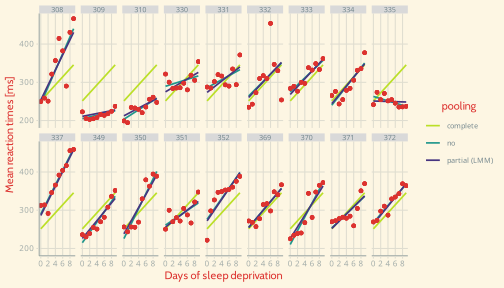
\includegraphics{20-SDT_files/figure-latex/unnamed-chunk-8-1} \end{center}

\chapter{Fitting Zipf's law to word frequency data}\label{fitting-zipfs-law-to-word-frequency-data}

Zipf's law predicts that the frequency of any word is inversely proportional to its rank in the frequency table. This phenomenon is observed across many natural languages and can be described by the Zipf-Mandelbrot law. Here I demonstrate how to apply maximum likelihood estimation and the binomial split approach, as described by Piantadosi \citep{PiantadosiZipf}, to fit Zipf's law to the word frequency data of ``Moby Dick''.

\section{Background}\label{background}

Zipf's law can be mathematically represented as:

\[ P(r) \propto \frac{1}{r^a} \]

where \(P(r)\) is the probability of the \(r\)-th most common word, and \(a\) is a parameter that typically lies close to 1 for natural language.

An extension of this is the Zipf-Mandelbrot law, which introduces a parameter \(s\) to account for a finite-size effect:

\[ P(r) \propto \frac{1}{(r+s)^a} \]

where \(s\) is a positive parameter that shifts the rank.

\section{Data preparation}\label{data-preparation}

We use the word frequency data from ``Moby Dick'' available in the \texttt{languageR} package. First, we load and clean the data:

\begin{Shaded}
\begin{Highlighting}[]
\CommentTok{\# Clean environment and set working directory}
\FunctionTok{rm}\NormalTok{(}\AttributeTok{list=}\FunctionTok{ls}\NormalTok{())}

\CommentTok{\# Load necessary libraries}
\FunctionTok{library}\NormalTok{(tidyverse)}
\CommentTok{\#\textgreater{} {-}{-} Attaching core tidyverse packages {-}{-}{-}{-} tidyverse 2.0.0 {-}{-}}
\CommentTok{\#\textgreater{} v dplyr     1.1.4     v readr     2.1.5}
\CommentTok{\#\textgreater{} v forcats   1.0.0     v stringr   1.5.1}
\CommentTok{\#\textgreater{} v ggplot2   3.5.1     v tibble    3.2.1}
\CommentTok{\#\textgreater{} v lubridate 1.9.3     v tidyr     1.3.1}
\CommentTok{\#\textgreater{} v purrr     1.0.2     }
\CommentTok{\#\textgreater{} {-}{-} Conflicts {-}{-}{-}{-}{-}{-}{-}{-}{-}{-}{-}{-}{-}{-}{-}{-}{-}{-}{-}{-}{-}{-} tidyverse\_conflicts() {-}{-}}
\CommentTok{\#\textgreater{} x dplyr::filter() masks stats::filter()}
\CommentTok{\#\textgreater{} x dplyr::lag()    masks stats::lag()}
\CommentTok{\#\textgreater{} i Use the conflicted package (\textless{}http://conflicted.r{-}lib.org/\textgreater{}) to force all conflicts to become errors}
\end{Highlighting}
\end{Shaded}

\begin{Shaded}
\begin{Highlighting}[]
\FunctionTok{library}\NormalTok{(languageR)}

\CommentTok{\# Load and prepare Moby Dick word frequency data}
\FunctionTok{data}\NormalTok{(moby)}
\NormalTok{words }\OtherTok{\textless{}{-}}\NormalTok{ moby[}\FunctionTok{which}\NormalTok{(moby }\SpecialCharTok{!=} \StringTok{""}\NormalTok{)]}

\CommentTok{\# create a table with word frequencies}
\NormalTok{word\_freq }\OtherTok{\textless{}{-}} \FunctionTok{table}\NormalTok{(words)}
\NormalTok{word\_freq\_df }\OtherTok{\textless{}{-}} \FunctionTok{as.data.frame}\NormalTok{(word\_freq, }\AttributeTok{stringsAsFactors=}\ConstantTok{FALSE}\NormalTok{)}
\FunctionTok{names}\NormalTok{(word\_freq\_df) }\OtherTok{\textless{}{-}} \FunctionTok{c}\NormalTok{(}\StringTok{"word"}\NormalTok{, }\StringTok{"frequency"}\NormalTok{)}
\FunctionTok{head}\NormalTok{(word\_freq\_df)}
\CommentTok{\#\textgreater{}       word frequency}
\CommentTok{\#\textgreater{} 1        {-}         3}
\CommentTok{\#\textgreater{} 2    {-}west         1}
\CommentTok{\#\textgreater{} 3  {-}wester         1}
\CommentTok{\#\textgreater{} 4 {-}Westers         1}
\CommentTok{\#\textgreater{} 5       [A         1}
\CommentTok{\#\textgreater{} 6  [SUDDEN         1}
\end{Highlighting}
\end{Shaded}

We then rank the words by frequency

\begin{Shaded}
\begin{Highlighting}[]
\NormalTok{ranked\_words }\OtherTok{\textless{}{-}}\NormalTok{ word\_freq\_df }\SpecialCharTok{\%\textgreater{}\%}
  \FunctionTok{arrange}\NormalTok{(}\FunctionTok{desc}\NormalTok{(frequency)) }\SpecialCharTok{\%\textgreater{}\%}
  \FunctionTok{mutate}\NormalTok{(}\AttributeTok{word =} \FunctionTok{factor}\NormalTok{(word, }\AttributeTok{levels =}\NormalTok{ word),}
         \AttributeTok{rank =} \FunctionTok{rank}\NormalTok{(}\SpecialCharTok{{-}}\NormalTok{frequency, }\AttributeTok{ties.method =} \StringTok{"random"}\NormalTok{))}
\end{Highlighting}
\end{Shaded}

\section{Estimation}\label{estimation}

We define custom functions for the binomial split, the negative log-likelihood, and the Zipf--Mandelbrot law probability mass function:

\begin{Shaded}
\begin{Highlighting}[]
\CommentTok{\# Binomial split {-} randomly split the corpus to ensure independence of rank and frequencies estimates}
\NormalTok{binomial\_split }\OtherTok{\textless{}{-}} \ControlFlowTok{function}\NormalTok{(data, }\AttributeTok{p=}\FloatTok{0.5}\NormalTok{)\{}
\NormalTok{  f1 }\OtherTok{\textless{}{-}} \FunctionTok{rep}\NormalTok{(}\ConstantTok{NA}\NormalTok{, }\FunctionTok{nrow}\NormalTok{(data))}
\NormalTok{  f2 }\OtherTok{\textless{}{-}} \FunctionTok{rep}\NormalTok{(}\ConstantTok{NA}\NormalTok{, }\FunctionTok{nrow}\NormalTok{(data))}
  \ControlFlowTok{for}\NormalTok{(i }\ControlFlowTok{in} \DecValTok{1}\SpecialCharTok{:}\FunctionTok{nrow}\NormalTok{(data))\{}
\NormalTok{    f1[i] }\OtherTok{\textless{}{-}} \FunctionTok{rbinom}\NormalTok{(}\DecValTok{1}\NormalTok{, }\AttributeTok{size=}\NormalTok{data}\SpecialCharTok{$}\NormalTok{frequency[i], }\AttributeTok{prob=}\NormalTok{p)}
\NormalTok{    f2[i] }\OtherTok{\textless{}{-}}\NormalTok{ data}\SpecialCharTok{$}\NormalTok{frequency[i] }\SpecialCharTok{{-}}\NormalTok{ f1[i] }
\NormalTok{  \}}
\NormalTok{  data\_split }\OtherTok{\textless{}{-}} \FunctionTok{data.frame}\NormalTok{(}
    \AttributeTok{word =}\NormalTok{ data}\SpecialCharTok{$}\NormalTok{word,}
    \AttributeTok{frequency =}\NormalTok{ f1,}
    \AttributeTok{rank =} \FunctionTok{rank}\NormalTok{(}\SpecialCharTok{{-}}\NormalTok{f2, }\AttributeTok{ties.method =} \StringTok{"random"}\NormalTok{)}
\NormalTok{  )}
  \FunctionTok{return}\NormalTok{(data\_split)}
\NormalTok{\}}

\CommentTok{\# negative log{-}likelihood function (for optimization)}
\NormalTok{neglog\_likelihood }\OtherTok{\textless{}{-}} \ControlFlowTok{function}\NormalTok{(params, data) \{}
\NormalTok{  s }\OtherTok{\textless{}{-}}\NormalTok{ params[}\DecValTok{1}\NormalTok{]}
\NormalTok{  a }\OtherTok{\textless{}{-}}\NormalTok{ params[}\DecValTok{2}\NormalTok{]}
  
\NormalTok{  N }\OtherTok{\textless{}{-}} \FunctionTok{length}\NormalTok{(data}\SpecialCharTok{$}\NormalTok{frequency)}
\NormalTok{  M }\OtherTok{\textless{}{-}} \FunctionTok{sum}\NormalTok{(data}\SpecialCharTok{$}\NormalTok{frequency)}
\NormalTok{  logP\_data }\OtherTok{\textless{}{-}}\NormalTok{ M}\SpecialCharTok{*}\FunctionTok{log}\NormalTok{(}\FunctionTok{sum}\NormalTok{(((}\DecValTok{1}\SpecialCharTok{:}\NormalTok{N)}\SpecialCharTok{+}\NormalTok{s)}\SpecialCharTok{\^{}}\NormalTok{(}\SpecialCharTok{{-}}\NormalTok{a)))}\SpecialCharTok{+}\NormalTok{a}\SpecialCharTok{*}\FunctionTok{sum}\NormalTok{(data}\SpecialCharTok{$}\NormalTok{frequency[data}\SpecialCharTok{$}\NormalTok{rank]}\SpecialCharTok{*}\FunctionTok{log}\NormalTok{(data}\SpecialCharTok{$}\NormalTok{rank}\SpecialCharTok{+}\NormalTok{s))}
  \FunctionTok{return}\NormalTok{(logP\_data)}
\NormalTok{\}}

\CommentTok{\# probability mass function for Zipf–Mandelbrot law}
\CommentTok{\# as defined in: https://en.wikipedia.org/wiki/Zipf\%E2\%80\%93Mandelbrot\_law}
\NormalTok{dzipf }\OtherTok{\textless{}{-}} \ControlFlowTok{function}\NormalTok{(rank, params, N)\{}
\NormalTok{  s }\OtherTok{\textless{}{-}}\NormalTok{ params[}\DecValTok{1}\NormalTok{]}
\NormalTok{  a }\OtherTok{\textless{}{-}}\NormalTok{ params[}\DecValTok{2}\NormalTok{]}
\NormalTok{  p }\OtherTok{\textless{}{-}}\NormalTok{ ((rank }\SpecialCharTok{+}\NormalTok{ s)}\SpecialCharTok{\^{}}\NormalTok{(}\SpecialCharTok{{-}}\NormalTok{a))}\SpecialCharTok{/}\NormalTok{(}\FunctionTok{sum}\NormalTok{((rank }\SpecialCharTok{+}\NormalTok{ s)}\SpecialCharTok{\^{}}\NormalTok{(}\SpecialCharTok{{-}}\NormalTok{a)))}
  \FunctionTok{return}\NormalTok{(p)}
\NormalTok{\}}
\end{Highlighting}
\end{Shaded}

We then fit the model using the \texttt{optim} function:

\begin{Shaded}
\begin{Highlighting}[]
\CommentTok{\# Initial parameter values for optimization}
\NormalTok{init\_params }\OtherTok{\textless{}{-}} \FunctionTok{c}\NormalTok{(}\AttributeTok{s =} \DecValTok{1}\NormalTok{, }\AttributeTok{a =} \DecValTok{1}\NormalTok{)}

\CommentTok{\# Fitting model to the data}
\NormalTok{fit\_zipf }\OtherTok{\textless{}{-}} \FunctionTok{optim}\NormalTok{(}\AttributeTok{par =}\NormalTok{ init\_params, }
                \AttributeTok{fn =}\NormalTok{ neglog\_likelihood, }
                \AttributeTok{data =}\NormalTok{ ranked\_words,}
                \AttributeTok{method =} \StringTok{"L{-}BFGS{-}B"}\NormalTok{, }
                \AttributeTok{lower =} \FunctionTok{c}\NormalTok{(}\DecValTok{0}\NormalTok{, }\DecValTok{0}\NormalTok{),}
                \AttributeTok{upper =} \FunctionTok{c}\NormalTok{(}\DecValTok{100}\NormalTok{, }\DecValTok{100}\NormalTok{),}
                \AttributeTok{hessian =} \ConstantTok{TRUE}\NormalTok{)}
\end{Highlighting}
\end{Shaded}

\section{Results}\label{results}

Here are the estimated values of the parameters \(s\) and \(a\)

\begin{Shaded}
\begin{Highlighting}[]
\FunctionTok{print}\NormalTok{(fit\_zipf}\SpecialCharTok{$}\NormalTok{par)}
\CommentTok{\#\textgreater{}        s        a }
\CommentTok{\#\textgreater{} 1.817667 1.072602}
\end{Highlighting}
\end{Shaded}

We can get standard errors of the parameters estimates from the Hessian matrix:

\begin{Shaded}
\begin{Highlighting}[]
\FunctionTok{sqrt}\NormalTok{(}\FunctionTok{diag}\NormalTok{(}\FunctionTok{solve}\NormalTok{(fit\_zipf}\SpecialCharTok{$}\NormalTok{hessian)))}
\CommentTok{\#\textgreater{}           s           a }
\CommentTok{\#\textgreater{} 0.032707787 0.001272293}
\end{Highlighting}
\end{Shaded}

Note that these standard errors do not take into account the additional sampling variability due to the binomial split. In order to take this into account we can re-estimate the model for multiple random splits, and examine how much parameters vary across spits.

\section{Visualization}\label{visualization}

Finally, we can visualize the fitted model against the actual data in the classical rank-frequency plot:

\begin{Shaded}
\begin{Highlighting}[]
\CommentTok{\#computed predicted probabilities}
\NormalTok{ranked\_words}\SpecialCharTok{$}\NormalTok{probability\_predicted }\OtherTok{\textless{}{-}} \FunctionTok{dzipf}\NormalTok{(}\AttributeTok{rank=}\NormalTok{ranked\_words}\SpecialCharTok{$}\NormalTok{rank, }
                                        \AttributeTok{params=}\NormalTok{fit\_zipf}\SpecialCharTok{$}\NormalTok{par,}
                                        \AttributeTok{N=}\FunctionTok{length}\NormalTok{(ranked\_words}\SpecialCharTok{$}\NormalTok{frequency))}

\CommentTok{\# Make rank{-}frequency plot using ggplo2}
\FunctionTok{ggplot}\NormalTok{() }\SpecialCharTok{+}
  \FunctionTok{geom\_point}\NormalTok{(}\AttributeTok{data=}\NormalTok{ranked\_words, }\AttributeTok{pch=}\DecValTok{21}\NormalTok{, }\AttributeTok{size=}\FloatTok{0.6}\NormalTok{,}
             \FunctionTok{aes}\NormalTok{(}\AttributeTok{x =}\NormalTok{ rank, }\AttributeTok{y =}\NormalTok{ frequency}\SpecialCharTok{/}\FunctionTok{sum}\NormalTok{(frequency))) }\SpecialCharTok{+}
  \FunctionTok{geom\_line}\NormalTok{(}\AttributeTok{data=}\NormalTok{ranked\_words,}
            \FunctionTok{aes}\NormalTok{(}\AttributeTok{x =}\NormalTok{ rank,}\AttributeTok{y =}\NormalTok{ probability\_predicted), }
            \AttributeTok{color=}\StringTok{"blue"}\NormalTok{) }\SpecialCharTok{+}
  \FunctionTok{scale\_x\_log10}\NormalTok{() }\SpecialCharTok{+}
  \FunctionTok{scale\_y\_log10}\NormalTok{() }\SpecialCharTok{+}
  \FunctionTok{theme\_bw}\NormalTok{() }\SpecialCharTok{+}
  \FunctionTok{labs}\NormalTok{(}
    \AttributeTok{title =} \StringTok{"Moby Dick"}\NormalTok{,}
    \AttributeTok{x =} \StringTok{"Rank (log scale)"}\NormalTok{,}
    \AttributeTok{y =} \StringTok{"Probability (log scale)"}
\NormalTok{  )}
\end{Highlighting}
\end{Shaded}

\begin{center}\includegraphics{21-zipf_files/figure-latex/unnamed-chunk-7-1} \end{center}

\chapter{Workshops}\label{workshops}

Either click on the links or click on the embedded slides and press `F' to go full screen. Advance through slides with arrow keys, and press `O' for an overview of all slides.

\section{Linear multilevel models (LMM) workshop (9th Sept 2022)}\label{linear-multilevel-models-lmm-workshop-9th-sept-2022}

\textbf{Part 1} (\href{https://mlisi.xyz/files/workshops/LMM101/LMM_part1.html}{link})

\textbf{Part 2} (\href{https://mlisi.xyz/files/workshops/LMM101/LMM_part2.html}{link})

\textbf{Practicals}

\href{https://mlisi.xyz/files/workshops/LMM101/exercises/exercises_questions.html}{Exercises with solution (link)}

\section{Introduction to meta-analyses in R}\label{introduction-to-meta-analyses-in-r}

22nd February 2023

(\href{https://mlisi.xyz/files/workshops/meta_analyses/meta_analyses_slides.html}{link})

\section{Power analyses via data simulation}\label{power-analyses-via-data-simulation}

15th November 2023

Links: (\href{https://mlisi.xyz/files/workshops/power_analyses/power_analyses.html}{slides}),
(\href{https://mlisi.xyz/files/workshops/power_analyses/power_analysis_workshop_script.R}{script})

\section{Introduction to Bayesian data analysis using R and Stan}\label{introduction-to-bayesian-data-analysis-using-r-and-stan}

29th November 2023

Link: (\href{https://mlisi.xyz/files/workshops/intro_bayes/intro-Bayes.html}{slides}),

See this Github repository for code examples and datasets: \url{https://github.com/mattelisi/intro-Bayes}.

\section{Introduction to causal reasoning with graphical models}\label{introduction-to-causal-reasoning-with-graphical-models}

15th January 2025

\url{https://mlisi.xyz/files/workshops/causal/RHUL_causal_intro.html}

Link: (\href{https://mlisi.xyz/files/workshops/causal/RHUL_causal_intro.html}{slides}),

\{\{\textless{} revealjs file=``\url{https://mlisi.xyz/files/workshops/causal/RHUL_causal_intro.html}'' height=``500px'' class=``ratio ratio-16x9'' \textgreater\}\}

\section{Introduction to linear algebra}\label{introduction-to-linear-algebra}

Lecture for MSc module PS5210 (version from: 7th December 2022)

\textbf{Part 2} (\href{https://mlisi.xyz/files/workshops/numerical_skills_lecture/slides_numerical_skills_part2.html}{link})

\chapter{Useful links \& resources}\label{useful-links-resources}

\section{Statistical theory}\label{statistical-theory}

\subsection{\texorpdfstring{\href{http://www.math.wm.edu/~leemis/chart/UDR/UDR.html}{Map of univariate statistical distributions}}{Map of univariate statistical distributions}}\label{map-of-univariate-statistical-distributions}

\includegraphics[width=0.75\textwidth,height=\textheight]{images/distributions_univariate_map.png}

  \bibliography{book.bib,packages.bib}

\end{document}
